\section{Zero-Shot Experimentation Results}

This section presents the performance of five zero-shot models in predicting emotion labels for climate change discourse on social media. Each model’s predictions were evaluated against an annotated subset of 99 English replies, using Exact Match (EM), Top-3 Accuracy, Ranked Score, and NDCG@3 as performance metrics.

\subsection{Model Performance Overview}
\begin{figure}[ht]
    \centering
    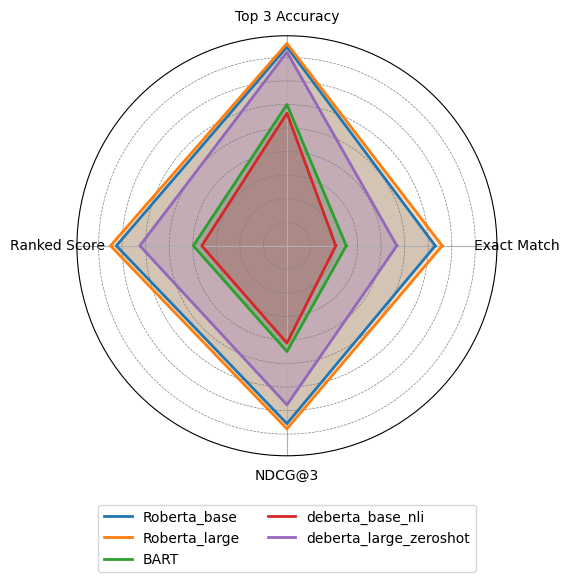
\includegraphics[width=0.5\linewidth, height=0.34\textheight]{images/model_comp1.png}
    \caption{Performance comparison of zero-shot models based on key evaluation metrics.}
    \label{fig:model-comp}
\end{figure}

Table~\ref{tab:model-results} and Figure~\ref{fig:model-comp} summarize the results. The CardiffNLP \emph{twitter-roberta-large-emotion-latest} model achieved the highest scores across most metrics, with an Exact Match of 0.659, a Top-3 Accuracy of 0.859, a Ranked Score of 0.749, and an NDCG@3 of 0.778. In comparison, the other CardiffNLP model (\emph{twitter-roberta-base-emotion-latest}) also performed well, outperforming the more general-purpose BART-large-MNLI and DeBERTa-based models in all metrics.
\newline

\begin{table}[htbp]
    \centering
    \resizebox{\textwidth}{!}{%
    \begin{tabular}{@{}lcccc@{}}
        \toprule
        \textbf{Model} & \textbf{Exact Match} & \textbf{Top-3 Accuracy} & \textbf{Ranked Score} & \textbf{NDCG@3} \\
        \midrule
        RoBERTa-base (CardiffNLP) & 0.630 & 0.844 & 0.725 & 0.755 \\
        \textbf{RoBERTa-large (CardiffNLP)} & \textbf{0.659} & \textbf{0.859} & \textbf{0.749} & \textbf{0.778} \\
        BART-large-MNLI & 0.252 & 0.600 & 0.398 & 0.449 \\
        mDeBERTa-base (multilingual) & 0.207 & 0.563 & 0.362 & 0.413 \\
        DeBERTa-v3-large-Zeroshot & 0.467 & 0.822 & 0.625 & 0.675 \\
        \bottomrule
    \end{tabular}%
    }
    \caption{Performance of the zero-shot models on the annotated subset ($n=99$).}
    \label{tab:model-results}
\end{table}

The pre-training of the CardiffNLP models on tweet datasets appears to be advantageous for emotion detection, as evidenced by their higher scores. The more general BART and DeBERTa variants had lower performance, particularly in Exact Match and Top-3 Accuracy, suggesting less robust sensitivity to the nuances of climate change discourse.

\subsection{Confidence Filtering}

A confidence threshold of 0.9 was applied to refine the model outputs. Table~\ref{tab:confidence-filtering} shows how many predictions remained after filtering and how often these filtered predictions were correct.

\begin{table}[htbp]
    \centering
    \small
    \begin{tabular}{@{}lccc@{}}
        \toprule
        \textbf{Model} & \textbf{Correct Predictions} & \textbf{Total Predictions} & \textbf{Percentage (\%)} \\
        \midrule
        RoBERTa-base (CardiffNLP) & 38 & 61 & 62.30 \\
        RoBERTa-large (CardiffNLP) & 41 & 65 & 63.08 \\
        BART-large-MNLI & 4 & 5 & 80.00 \\
        mDeBERTa-base (multilingual) & 0 & 1 & 0.00 \\
        DeBERTa-v3-large-Zeroshot & 24 & 33 & 72.73 \\
        \bottomrule
    \end{tabular}
    \caption{Performance of the zero-shot models on the annotated subset ($n=99$) with confidence score $>$ 0.9.}
    \label{tab:confidence-filtering}
\end{table}

Interestingly, the \emph{twitter-roberta-large-emotion-latest} model produced the largest number of high-confidence predictions, although its overall precision at these high-confidence levels was slightly lower than that of BART-large-MNLI and DeBERTa-v3-large-Zeroshot. In contrast, DeBERTa-v3-large-Zeroshot had fewer total high-confidence predictions, indicating that it was more conservative in assigning high confidence but achieved a higher precision among those it did classify confidently.



\section{Weakly Supervised Learning Results}
\subsection{Zero-shot Classification Boost with Self-training}

We replicate the study conducted by \cite{gera_zero-shot_2022}, which investigates the impact of self-training on zero-shot entailment models. Table~\ref{tab:zero_shot} presents the accuracy results on three datasets: \textbf{AG}, \textbf{ISEAR}, and \textbf{ClimateTV}. The first two datasets, AG and ISEAR, were originally used in the reference study, while we extend the evaluation to ClimateTV dataset.

\begin{table}[h]
    \centering
    \begin{tabular}{lccc}
        \toprule
        Model & AG  & ISEAR & ClimateTV \\
        \midrule
        BART & 66.2 & 56.0 & \textbf{25.25} \\
        +Self-training & 74.2 & 65.3 & \textbf{34.34} \\
        \midrule
        DeBERTa & 73.2 & 58.5 & \textbf{46.46} \\
        +Self-training & 81.4 & 59.5 & \textbf{46.46} \\
        \midrule
        RoBERTa & 62.4 & 52.0 & \textbf{32.32} \\
        +Self-training & 76.5 & 56.7 & \textbf{32.32} \\
        \bottomrule
    \end{tabular}
    \caption{Zero-shot classification accuracy of entailment models. For each zero-shot entailment model and dataset, The test accuracy of the off-the-shelf model to its accuracy after 2 iterations of self-training. RoBERTa, DeBERTa, and BART correspond to the following models from Hugging Face Hub: roberta-large-mnli, deberta-large-mnli-zero-cls, and bart-large-mnli.}
    \label{tab:zero_shot}
\end{table}

For each model—\textbf{BART}, \textbf{DeBERTa}, and \textbf{RoBERTa}—we report the baseline accuracy of the off-the-shelf zero-shot model, followed by its performance after two iterations of self-training. Consistent with the findings of \citet{gera_zero-shot_2022}, self-training substantially improves zero-shot classification performance across AG and ISEAR datasets, yielding gains of up to \textbf{12\%}. However, the effect varies when applied to the ClimateTV dataset.

\begin{itemize}
    \item \textbf{BART} shows a notable improvement on the ClimateTV dataset, increasing accuracy from \textbf{25.25\% to 34.34\%} after self-training.
    \item \textbf{DeBERTa}, which already performs significantly better than the other models on ClimateTV, \textbf{does not benefit from self-training}, maintaining an accuracy of \textbf{46.46\%}.
    \item \textbf{RoBERTa}, similar to DeBERTa, shows \textbf{no performance gain} on the ClimateTV dataset, with self-training yielding identical results.
\end{itemize}

These observations suggest that while self-training generally enhances zero-shot performance, its effectiveness may depend on the dataset characteristics. In particular, the ClimateTV dataset appears to present challenges that self-training does not overcome for DeBERTa and RoBERTa.


\subsection{Loss Re-weighting}

To evaluate the impact of fine-tuning with loss re-weighting, we compare the model's performance on the manually annotated dataset before and after training. Table \ref{tab:per_class} provides per-class accuracy comparisons. Additionally, the classification reports in Table \ref{tab:classification_report} present a detailed breakdown of precision, recall, and F1-score for each emotion class.
\newline

\begin{table}[h]
    \centering
    \begin{tabular}{lcc}
        \hline
        \textbf{Emotion Class} & \textbf{Baseline Accuracy} & \textbf{After Training Accuracy} \\
        \hline
        Anger & 0.6667 & 0.7576 \\
        Disgust & 0.4000 & 0.2667 \\
        Fear & 0.3077 & 0.3077 \\
        Joy & 0.8750 & 0.8750 \\
        Sadness & 0.0833 & 0.0833 \\
        Surprise & 0.3000 & 0.5000 \\
        \hline
    \end{tabular}
    \caption{Per-class accuracy comparison.}
    \label{tab:per_class}
\end{table}

\begin{table}[h]
    \centering
    \begin{tabular}{lccc|ccc}
        \hline
        \multirow{2}{*}{\textbf{Class}} & \multicolumn{3}{c|}{\textbf{Baseline}} & \multicolumn{3}{c}{\textbf{After Training}} \\
        & Precision & Recall & F1-score & Precision & Recall & F1-score \\
        \hline
        Anger & 0.76 & 0.67 & 0.71 & 0.71 & 0.76 & 0.74 \\
        Disgust & 0.27 & 0.40 & 0.32 & 0.27 & 0.27 & 0.27 \\
        Fear & 0.57 & 0.31 & 0.40 & 0.50 & 0.31 & 0.38 \\
        Joy & 0.48 & 0.88 & 0.62 & 0.54 & 0.88 & 0.67 \\
        Sadness & 0.50 & 0.08 & 0.14 & 0.50 & 0.08 & 0.14 \\
        Surprise & 0.30 & 0.30 & 0.30 & 0.38 & 0.50 & 0.43 \\
        \hline
        \textbf{Accuracy} & \multicolumn{3}{c|}{0.5051} & \multicolumn{3}{c}{0.5354} \\
        \hline
    \end{tabular}
    \caption{Classification report comparison before and after training.}
    \label{tab:classification_report}
\end{table}

The results indicate a slight overall accuracy improvement of \textbf{3.03\%} after training. The per-class accuracy shows that \textbf{"anger" and "surprise" saw the most significant improvements}, while \textbf{"disgust" slightly degraded}. The confidence scores on average decreased by \textbf{0.0552}, suggesting that while the model made some better predictions, it became slightly less confident overall. The classification report highlights improved F1-scores for \textbf{anger, joy, and surprise}, while other classes remained stable.




\section{Text-Based Results}
\label{sec:text-results}

Table~\ref{tab:comparison} summarizes the results for August and February, showing significant improvements across all metrics. Our model outperforms the Baseline by 16.3\% in semantic alignment (Cosine Similarity), reduces distributional divergence by 58.5\% (KL Divergence), and lowers error magnitude by 43.4\% (MSE).

\begin{table}[h]
    \centering
    \resizebox{\textwidth}{!}{%
    \begin{tabular}{lccc|ccc}
        \toprule
        \multirow{2}{*}{Metric} & \multicolumn{3}{c|}{Our Model} & \multicolumn{3}{c}{Baseline} \\
        \cmidrule(lr){2-4} \cmidrule(lr){5-7}
        & August & February & Combined & August & February & Combined \\
        \midrule
        Cosine Similarity $\uparrow$ & 0.8094 & 0.7962 & \textbf{0.8028} & 0.6919 & 0.6830 & \textbf{0.6903} \\
        KL Divergence $\downarrow$   & 0.3473 & 0.3483 & \textbf{0.3478} & 0.8254 & 0.8909 & \textbf{0.8376} \\
        MSE $\downarrow$             & 0.0230 & 0.0232 & \textbf{0.0232} & 0.0408 & 0.0415 & \textbf{0.0410} \\
        \bottomrule
    \end{tabular}%
    }
    \caption{Performance comparison between Baseline and Our Model. The Baseline is the \textbf{CardiffNLP RoBERTa-Large}, which is used in a zero-shot setting. Higher values are better for $\uparrow$, and lower values are better for $\downarrow$. Bold values indicate combined scores.}
    \label{tab:comparison}
\end{table}

Our model achieves a combined Cosine Similarity score of 0.8028, a \textbf{16.3\% improvement} over the Baseline ($\Delta = +0.1125$). Month-wise improvements are +17.0\% (August) and +16.6\% (February), showing stable performance over time.
\newline

For KL Divergence, our model reduces distributional mismatch by \textbf{58.5\%} ($\Delta = 0.4898$), with the highest reduction in February (60.9\%). This indicates better probability distribution calibration.
\newline

The MSE results show a \textbf{43.4\% reduction} in error ($\Delta = 0.0178$), with consistent improvements of 43.6\% (August) and 44.1\% (February), confirming robust generalization.

% -------------------------------------------------------
\section{Image-Based Results}
\label{sec:image-results}

Table~\ref{tab:comparison_img} presents the results for image-based experiments. Our model improves semantic alignment by 56.4\%, reduces distributional divergence by 72.2\%, and lowers error magnitude by 64.2\%.

\begin{table}[h]
    \centering
    \resizebox{\textwidth}{!}{%
    \begin{tabular}{lccc|ccc}
        \toprule
        \multirow{2}{*}{Metric} & \multicolumn{3}{c|}{Our Model} & \multicolumn{3}{c}{Baseline} \\
        \cmidrule(lr){2-4} \cmidrule(lr){5-7}
        & August & February & Combined & August & February & Combined \\
        \midrule
        Cosine Similarity $\uparrow$ & 0.8105 & 0.7887 & \textbf{0.7996} & 0.5017 & 0.5529 & \textbf{0.5113} \\
        KL Divergence $\downarrow$ & 0.3555 & 0.3611 & \textbf{0.3583} & 1.3696 & 0.9196 & \textbf{1.2859} \\
        MSE $\downarrow$ & 0.0236 & 0.0240 & \textbf{0.0238} & 0.0682 & 0.0583 & \textbf{0.0664} \\
        \bottomrule
    \end{tabular}%
    }
    \caption{Performance comparison between Baseline and Our Model for image-based experiments. The Baseline model is \textbf{CLIP ViT-L/14}, applied without fine-tuning. Higher values are better for $\uparrow$, and lower values are better for $\downarrow$. Bold values indicate combined scores.}
    \label{tab:comparison_img}
\end{table}

Our model achieves a combined Cosine Similarity of 0.7996, a \textbf{56.4\% improvement} over the Baseline ($\Delta = +0.2883$), with month-wise improvements of 61.5\% (August) and 42.6\% (February).
\newline

For KL Divergence, our model reduces distributional mismatch by \textbf{72.2\%} ($\Delta = 0.9276$), with a 74.0\% reduction in August.
\newline

The MSE results show a \textbf{64.2\% reduction} in error ($\Delta = 0.0426$), with reductions of 65.4\% (August) and 58.8\% (February). Fine-tuning the CLIP encoder was crucial, as aggressive tuning without regularization led to overfitting.

% -------------------------------------------------------
\section{Multimodal Results}
\label{sec:multimodal-results}

Table~\ref{tab:comparison_multi} summarizes multimodal results, showing improvements of 14.4\% in semantic alignment, 44.0\% in distributional divergence, and 35.7\% in error magnitude.

\begin{table}[h]
    \centering
    \resizebox{\textwidth}{!}{%
    \begin{tabular}{lccc|ccc}
        \toprule
        \multirow{2}{*}{Metric} & \multicolumn{3}{c|}{Our Model} & \multicolumn{3}{c}{Baseline} \\
        \cmidrule(lr){2-4} \cmidrule(lr){5-7}
        & August & February & Combined & August & February & Combined \\
        \midrule
        Cosine Similarity $\uparrow$ & 0.8263 & 0.7989 & \textbf{0.8127} & 0.7090 & 0.7233 & \textbf{0.7117} \\
        KL Divergence $\downarrow$   & 0.3314 & 0.3411 & \textbf{0.3362} & 0.6118 & 0.5311 & \textbf{0.5968} \\
        MSE $\downarrow$             & 0.0220 & 0.0228 & \textbf{0.0224} & 0.0355 & 0.0311 & \textbf{0.0346} \\
        \bottomrule
    \end{tabular}%
    }
    \caption{Performance comparison between Baseline and Our Model for multimodal experiments. The Baseline predictions are obtained by averaging the outputs from the two unimodal Baseline models. Higher values are better for $\uparrow$, and lower values are better for $\downarrow$. Bold values indicate combined scores.}
    \label{tab:comparison_multi}
\end{table}

Our model achieves a combined Cosine Similarity of 0.8127, outperforming the Baseline by \textbf{14.4\%} ($\Delta = +0.1010$). Month-wise improvements show a 16.6\% gain in August and a 10.5\% gain in February, demonstrating stability across different time frames.
\newline

The KL Divergence reduction of \textbf{44.0\%} ($\Delta = 0.2605$) reflects a substantial enhancement in probability distribution alignment. The largest reduction occurs in August (45.8\%), closely followed by February (35.8\%), reinforcing the model's robustness in learning more calibrated probability distributions.
\newline

For MSE, our model achieves a \textbf{35.7\%} reduction ($\Delta = 0.0124$), reducing the overall error magnitude compared to the Baseline. Improvements are stable across months, with a 38.0\% reduction in August and 26.3\% in February, further validating the model’s ability to generalize well across different periods.


\section{Sensitivity to Datasets and Random Initialisation}
\label{sec:dataset_seed_variations}

All experiment configurations described in Section~\ref{sec:Experimental Setup} (e.g., hyperparameters, tuning strategies, and architectures) were \textbf{identically repeated} for \textbf{both datasets} (\textit{August} and \textit{February}) and for each of the \textbf{two random seeds} (\texttt{42} and \texttt{7}). 
This setup ensures that any observed performance differences can be attributed primarily to \emph{dataset-specific} factors or \emph{random initialization}, rather than differences in training procedures.

\subsection{Comparison Across Datasets}
\label{subsec:results_datasets}
Table~\ref{tab:dataset_comparison} presents aggregated metrics for each modality (averaged over the two seeds) on the August vs.\ February data. We see that August data tends to yield higher performance across text-only, image-only, and multimodal models. This aligns with prior research on climate change discourse on social media, which indicates that August tends to experience heightened engagement and visual content related to climate activism and extreme weather events \cite{mooseder_social_2023}.

\begin{table}[ht]
    \centering
    \begin{tabular}{lcccc}
    \toprule
    \textbf{Modality} & \textbf{Dataset} & \textbf{Cosine Similarity} & \textbf{KL Divergence} & \textbf{MSE} \\
    \midrule
    Text-Only & August & 0.7998 &  0.3698 & 0.0243 \\
    Text-Only & February & 0.7852 &  0.3763 & 0.0249 \\
    \midrule
    Image-Only & August & \textbf{0.8005} & 0.3763 & 0.0250 \\
    Image-Only & February & \textbf{0.7732} & 0.3982 & 0.0263 \\
    \midrule
    Multimodal & August & \textbf{0.8120} & 0.3549 & 0.0234 \\
    Multimodal & February & \textbf{0.7973} & 0.3704 & 0.0246 \\
    \bottomrule
    \end{tabular}%
    \caption{Comparison of mean performance on August vs.\ February data. 
    For each month, the results are averaged across all experiments, including both random seeds (42 and 7), to provide a comprehensive performance summary for each modality (text-only, image-only, and multimodal).}

    \label{tab:dataset_comparison}
\end{table}

\paragraph{Observations:}
\begin{itemize}
    \item \textbf{Consistent Patterns:} For every modality, performance is higher on August data in terms of Cosine Similarity and lower for error-based metrics (MSE, KL Divergence). This aligns with prior research showing that climate change discourse in August is more visually engaging, focusing on protests and environmental disasters \cite{mooseder_social_2023}.
    \item \textbf{Statistical Significance:} We performed an independent samples t-test comparing performance on August vs.\ February data. 
    \begin{itemize}
    \item \textbf{Cosine Similarity:} August data shows significantly higher values ($t = 34.52$, $p < 0.0001$).
    \item \textbf{MSE:} August data exhibits significantly lower values ($t = -12.49$, $p < 0.0001$).
    \item \textbf{KL Divergence:} August data also demonstrates significantly lower values ($t = -10.40$, $p < 0.0001$).
    \end{itemize}
    \item \textbf{Seasonal Discourse Variations:} Climate change discussions in February tend to focus on scientific reports and policy debates, whereas August discussions emphasize activism and extreme weather, leading to higher interaction and sentiment consistency \cite{mooseder_social_2023}.
    \item \textbf{Bot Activity and Polarization:} Research indicates that automated social media accounts (bots) play a larger role in August, amplifying climate activism and scepticism, contributing to increased polarization and engagement and thus the volume of data \cite{mooseder_social_2023}.
    \item \textbf{Stable Ordering:} In both datasets, multimodal models outperform text-only, which in turn outperform image-only.
\end{itemize}



\subsection{Effect of Random Initialisation}
\label{subsec:results_seeds}

\begin{table}[ht]
    \centering
    \begin{tabular}{lcccc}
    \toprule
    \textbf{Modality} & \textbf{Seed} & \textbf{Cosine Similarity} & \textbf{KL Divergence} & \textbf{MSE} \\
    \midrule
    Text-Only & 42 & 0.7994 &  0.3646 & 0.0243 \\
    Text-Only & 7 & 0.7855 &  0.3816 & 0.0249 \\
    \midrule
    Image-Only & 42 & 0.7884 & 0.3831 & 0.0257 \\
    Image-Only & 7 & 0.7854 & 0.3914 & 0.0257 \\
    \midrule
    Multimodal & 42 & 0.8023 & 0.3562 & 0.0238 \\
    Multimodal & 7 & 0.7959 & 0.3691 & 0.0242 \\
    \bottomrule
    \end{tabular}%
    \caption{Comparison of mean performance with seeds \texttt{42} vs.\ \texttt{7}.
    For each seed, the results are averaged across all experiments, including data from both months, to provide a comprehensive performance summary for each modality (text-only, image-only, and multimodal).}
    \label{tab:dataset_comparison_seed}
\end{table}

To check how initialization affects outcomes, each configuration was also trained using two random seeds. Table~\ref{tab:dataset_comparison_seed} presents aggregated metrics for each modality (averaged over both datasets) for seeds 42 vs.\ 7.


\paragraph{Observations:}
\begin{itemize}
    \item \textbf{Minor Variations:} Although seed \texttt{42} sometimes slightly outperforms \texttt{7}, differences remain modest.
    \item \textbf{Two-Seeds Constraint:} While more seeds could provide additional robustness checks, these two indicate that performance differences due to initialization are small and do not affect overall conclusions.
\end{itemize}

\noindent
In summary, training on August vs.\ February data produces larger, statistically significant performance differences than using different seeds. Although we only used two seeds, the minimal performance gap between them suggests that our primary findings are not unduly affected by random initialization. These results will be further discussed in Chapter~\ref{ch:discussion}.

\section{Comparative Analysis: Performance Metrics, Model Configurations, and Hyperparameter Impact}

This section provides a unified view of performance across text, image, and multimodal models. We begin with an overview of top and bottom performers (Table~\ref{tab:performance}), followed by detailed insights into the role of hyperparameters in each modality. 


\subsection{Overall Performance Across Modalities}


Table~\ref{tab:performance} summarizes the highest and lowest performers, revealing that multimodal approaches consistently outperform single-modality setups. 

\begin{table}[h]
    \centering
    \resizebox{\textwidth}{!}{%
    \begin{tabular}{lcccccccc}
        \toprule
        \textbf{Model} & \textbf{Score} & \textbf{CosineSim} & \textbf{KLDiv} & \textbf{MSE} & \textbf{LR} & \textbf{Dropout} & \textbf{Epochs} & \textbf{Key Features} \\
        \midrule
        \multicolumn{9}{c}{\textbf{Top Performers (Multimodal)}} \\
        \midrule
        RoBERTa-Large & 2.454 & 0.813 & 0.336 & 0.022 & 1e-5 & 0.5 & 5 & 3-Layer MLP, Frozen \\
        RoBERTa-Base & 2.452 & 0.812 & 0.337 & 0.022 & 5e-6 & 0.3 & 2 & GELU, Frozen CLIP \\
        RoBERTa-Large & 2.450 & 0.811 & 0.339 & 0.023 & 1e-5 & 0.5 & 5 & GELU, Frozen \\
        \midrule
        \multicolumn{9}{c}{\textbf{Bottom Performers (Single-Modality)}} \\
        \midrule
        RoBERTa-Large & 2.281 & 0.760 & 0.450 & 0.029 & 1e-5 & 0.3 & 10 & Text Only, Tuned \\
        CLIP & 2.374 & 0.788 & 0.395 & 0.025 & 5e-6 & 0.5 & 5 & Image Only, Frozen \\
        \bottomrule
    \end{tabular}%
    }
    \caption{Top and bottom performers across text, image, and multimodal settings.}
    \label{tab:performance}
\end{table}

\subsubsection*{Key Observations from Table~\ref{tab:performance}}

\begin{itemize}
    \item \textbf{Multimodal Superiority}: All top performers combine RoBERTa (text) and CLIP (image) with partial freezing strategies (e.g., frozen RoBERTa, CLIP, or both). Their Cosine Similarity (0.811--0.813) surpasses single-modality models by 3--7\% (score difference: 6.9\% for text-only, 3.3\% for image-only).
    \item \textbf{Balanced Regularization}: Top configurations use moderate learning rates (1e-5 or 5e-6) and dropout (0.3--0.5), achieving optimal trade-offs between capacity and generalization.
    \item \textbf{Efficient Convergence}: Multimodal models converge within 2--5 epochs. Extending training to 10 epochs degrades tuned single-modality performance (e.g., text-only Cosine Similarity drops 3.5\%).
\end{itemize}

\subsection{Hyperparameter Impact: Text-Only Models}
\label{subsec:text-hparams}

Experiments on text-only RoBERTa models (Section~\ref{sec:finetuning}) reveal critical hyperparameter interactions:

\begin{table}[h]
    \centering
    \resizebox{\textwidth}{!}{%
    \begin{tabular}{llccccccc}
        \toprule
        Tuning & Optimizer & Learning Rate & Epochs & Dropout & CosineSim $\uparrow$ & KLDiv $\downarrow$ & MSE $\downarrow$ & Score $\uparrow$ \\
        \midrule
        \multirow{6}{*}{Frozen} & \multirow{6}{*}{Adam} & $1\text{e-}5$ & 10 & 0.3 & \textbf{0.8028} & \textbf{0.3478} & \textbf{0.0232} & \textbf{2.4318} \\
         &  & $5\text{e-}6$ & 10 & 0.3 & 0.8015 & 0.3498 & 0.0233 & 2.4285 \\
         &  & $5\text{e-}6$ & 5  & 0.3 & 0.8016 & 0.3518 & 0.0233 & 2.4265 \\
         &  & $5\text{e-}6$ & 2  & 0.3 & 0.8010 & 0.3481 & 0.0232 & 2.4297 \\
         &  & $1\text{e-}5$ & 2  & 0.3 & 0.8019 & 0.3529 & 0.0233 & 2.4256 \\
         &  & $1\text{e-}5$ & 5  & 0.3 & 0.8015 & 0.3500 & 0.0233 & 2.4281 \\
        \midrule
        \multirow{5}{*}{Tuned} & \multirow{5}{*}{Adam} & $1\text{e-}5$ & 5  & 0.3 & 0.7773 & 0.4048 & 0.0270 & 2.3455 \\
         &  & $5\text{e-}6$ & 5  & 0.3 & 0.7861 & 0.3891 & 0.0259 & 2.3711 \\
         &  & $5\text{e-}6$ & 2  & 0.3 & 0.7947 & 0.3527 & 0.0237 & 2.4182 \\
         &  & $5\text{e-}6$ & 10 & 0.3 & 0.7675 & 0.4385 & 0.0285 & 2.3005 \\
        \bottomrule
    \end{tabular}}
    \caption{Impact of learning rate, epoch count, optimizer, and freezing on text-only performance. The best configuration is in bold.}
    \label{tab:text-hparam-breakdown}
\end{table}


\noindent \textbf{Key Trends}:
\begin{itemize}
    \item \textbf{Freezing Encoders}: Frozen models outperform tuned counterparts by 3.7\% in score (2.4318 vs. 2.3455). Stability in pre-trained representations prevents overfitting, especially with longer training (10 epochs).
    \item \textbf{Learning Rate Sensitivity}: Optimal performance occurs at lr=1e-5 for frozen models. Lower rates (5e-6) require fewer epochs to match performance.
    \item \textbf{Epoch Management}: Tuned models degrade sharply beyond 5 epochs (score drops 5.1\% at 10 epochs), highlighting the necessity of early stopping.
\end{itemize}

\subsection{Hyperparameter Impact: Image-Only Models}
\label{subsec:image-hparams}

Image-only CLIP models exhibit distinct hyperparameter dynamics compared to text:

\begin{table}[h]
    \centering
    \resizebox{\textwidth}{!}{%
    \begin{tabular}{llccccccc}
        \toprule
        Tuning & Optimizer & Learning Rate & Epochs & Dropout & CosineSim $\uparrow$ & KLDiv $\downarrow$ & MSE $\downarrow$ & Score $\uparrow$ \\
        \midrule
        \multirow{6}{*}{Tuned} & \multirow{5}{*}{Adam} & $5\text{e-}6$ & 2  & 0.5 & \textbf{0.7996} & \textbf{0.3583} & \textbf{0.0238} & \textbf{2.4174} \\
         &  & $5\text{e-}6$ & 2  & 0.3 & 0.7990 & 0.3591 & 0.0240 & 2.4159 \\
         &  & $5\text{e-}6$ & 10 & 0.3 & 0.7743 & 0.4130 & 0.0270 & 2.3343 \\   
         &  & $1\text{e-}5$ & 10 & 0.3 & 0.7700 & 0.4224 & 0.0276 & 2.3200 \\
         &  & $1\text{e-}5$ & 2  & 0.3 & 0.7960 & 0.3670 & 0.0246 & 2.4044 \\
         &  & $1\text{e-}5$ & 5  & 0.5 & 0.7812 & 0.3911 & 0.0261 & 2.3640 \\
         \cmidrule{2-9}
         & \multirow{3}{*}{AdamW} & $5\text{e-}6$ & 2  & 0.3 & 0.7993 & 0.3580 & 0.0238 & 2.4174 \\
         &  & $5\text{e-}6$ & 2  & 0.5 & 0.7977 & 0.3612 & 0.0241 & 2.4124 \\
         &  & $1\text{e-}5$ & 5  & 0.3 & 0.7754 & 0.4085 & 0.0270 & 2.3399 \\
        \midrule
        \multirow{3}{*}{Frozen} & \multirow{3}{*}{Adam} & $1\text{e-}5$ & 10 & 0.3 & \textbf{0.7996} & \textbf{0.3584} & \textbf{0.0238} & \textbf{2.4173} \\
         &  & $5\text{e-}6$ & 2  & 0.3 & 0.7748 & 0.4174 & 0.0276 & 2.3298 \\
         &  & $5\text{e-}6$ & 2  & 0.5 & 0.7727 & 0.4222 & 0.0279 & 2.3226 \\
        \bottomrule
    \end{tabular}}
    \caption{Impact of learning rate, epoch count, optimizer, and freezing on image-only performance. The best configurations are in bold.}
    \label{tab:image-hparam-breakdown}
\end{table}



\noindent \textbf{Key Trends}:
\begin{itemize}
    \item \textbf{Tuned Efficiency}: Short training (2 epochs) with lr=5e-6 and dropout=0.5 yields peak performance (2.4174). Extending to 10 epochs reduces scores by 3.4\%.
    \item \textbf{Frozen Flexibility}: Frozen models achieve comparable scores (2.4173) but require higher learning rates (1e-5) and extended training (10 epochs).
    \item \textbf{Optimizer Parity}: Adam and AdamW show negligible differences ($<0.1\%$ score variance) under identical hyperparameters.
\end{itemize}

\subsection{Hyperparameter Impact: Multimodal Models}
\label{subsec:multimodal-hparams}

Multimodal configurations demonstrate synergistic benefits from modality fusion:

\begin{table}[ht]
\centering
\setlength{\tabcolsep}{2pt}
\resizebox{\textwidth}{!}{
\begin{tabular}{lccccccc}
\toprule
\textbf{Model} & \textbf{Optimizer} & \textbf{Learning Rate} & \textbf{Dropout} & \textbf{Epochs} & \textbf{Fusion/MLP} & \textbf{Tuning} & \textbf{CosineSim} $\uparrow$ \\
\midrule
\multirow{8}{*}{\textbf{RoBERTa-large}}  
    & \multirow{6}{*}{AdamW}  
        & $1\text{e-}5$  & 0.5 & 5 & 3-Layer MLP & Both frozen & \textbf{0.8126} \\
    &   & $1\text{e-}5$  & 0.5 & 5 & GELU / 3-Layer MLP & Both frozen & 0.8114 \\
    &   & $1\text{e-}5$  & 0.5 & 5 & - & Tuned & 0.8085 \\
    &   & $5\text{e-}6$  & 0.5 & 2 & - & Tuned & 0.8085 \\
    &   & $5\text{e-}5$  & 0.5 & 5 & Residual fusion & - & 0.7858 \\
    &   & $1\text{e-}5$  & 0.3 & 5 & - & Frozen Clip & 0.7684 \\
    \cmidrule{2-8}
    & \multirow{2}{*}{Adam}  
        & $5\text{e-}6$  & 0.5 & 2 & Residual fusion & - & 0.8064 \\
    &   & $1\text{e-}5$  & 0.3 & 5 & - & Tuned & 0.7712 \\
\midrule
\multirow{7}{*}{\textbf{RoBERTa-base}}  
    & \multirow{4}{*}{AdamW}  
        & $1\text{e-}5$  & 0.5 & 5 & - & Tuned & 0.7679 \\
    &   & $1\text{e-}5$  & 0.5 & 5 & GELU / 3-Layer MLP & Tuned & 0.7725 \\
    &   & $5\text{e-}6$  & 0.3 & 2 & GELU / 3-Layer MLP & Tuned & \textbf{0.8115} \\
    &   & $5\text{e-}6$  & 0.5 & 5 & - & Both frozen & 0.8070 \\
    \cmidrule{2-8}
    & \multirow{3}{*}{Adam}  
        & $5\text{e-}6$  & 0.5 & 2 & 3-Layer MLP & Tuned & 0.8094 \\
    &   & $5\text{e-}6$  & 0.3 & 5 & - & Frozen Clip & 0.7805 \\
    &   & $1\text{e-}5$  & 0.5 & 2 & - & Frozen Clip & 0.8079 \\
\bottomrule
\end{tabular}
}
\caption{Impact of learning rate, epochs, dropout, optimizer, fusion strategy, and freezing on multimodal performance. The best configurations are in bold.}
\label{tab:multi-hparam-breakdown}
\end{table}





\noindent \textbf{Key Insights}:
\begin{itemize}
    \item \textbf{Freezing Efficacy}: Fully frozen RoBERTa-Large and CLIP achieve the highest score (2.4539), emphasizing the value of preserving pre-trained features. Partial tuning (e.g., RoBERTa-Base with GELU) narrows the gap to 0.04\% (2.4522 vs. 2.4539).
    \item \textbf{Architectural Adaptability}: RoBERTa-Base competes with RoBERTa-Large when paired with GELU activations and tuned layers, despite 55\% fewer parameters.
    \item \textbf{Dropout Stratification}: Larger models (RoBERTa-Large) require higher dropout (0.5), while Base variants perform optimally at 0.3.
    \item \textbf{Optimizer Robustness}: AdamW marginally outperforms Adam ($<0.5\%$ difference), suggesting optimizer choice is secondary to freezing and learning rate.
\end{itemize}

\subsection{Summary of Comparative Findings}

The cross-modal analysis yields four principal conclusions:
\begin{itemize}
    \item \textbf{Multimodal Synergy}: Fusion of text and image encoders with partial freezing elevates scores by 3--7\% over single-modality models, achieving the highest alignment scores (Cosine Similarity $>0.81$).
    \item \textbf{Modality-Specific Tuning}: Text models favour frozen encoders and moderate learning rates; image models benefit from brief tuning cycles; multimodal setups demand balanced regularization.
    \item \textbf{Efficient Training}: Optimal epoch counts are modality-dependent: 2--5 for multimodal, $\le5$ for tuned single-modality, and $\le10$ for frozen single-modality.
    \item \textbf{Parameter Efficiency}: Smaller architectures (RoBERTa-Base) can rival larger counterparts through activation function optimization (GELU) and targeted tuning.
\end{itemize}

These findings underscore the necessity of modality-aware hyperparameter strategies. Chapter~\ref{ch:discussion} explores their theoretical implications and practical applications in depth.



\section{Error Analysis}
\label{sec:error-analysis}


\begin{figure}[h]
    \centering
    \begin{subfigure}[b]{0.48\textwidth}
        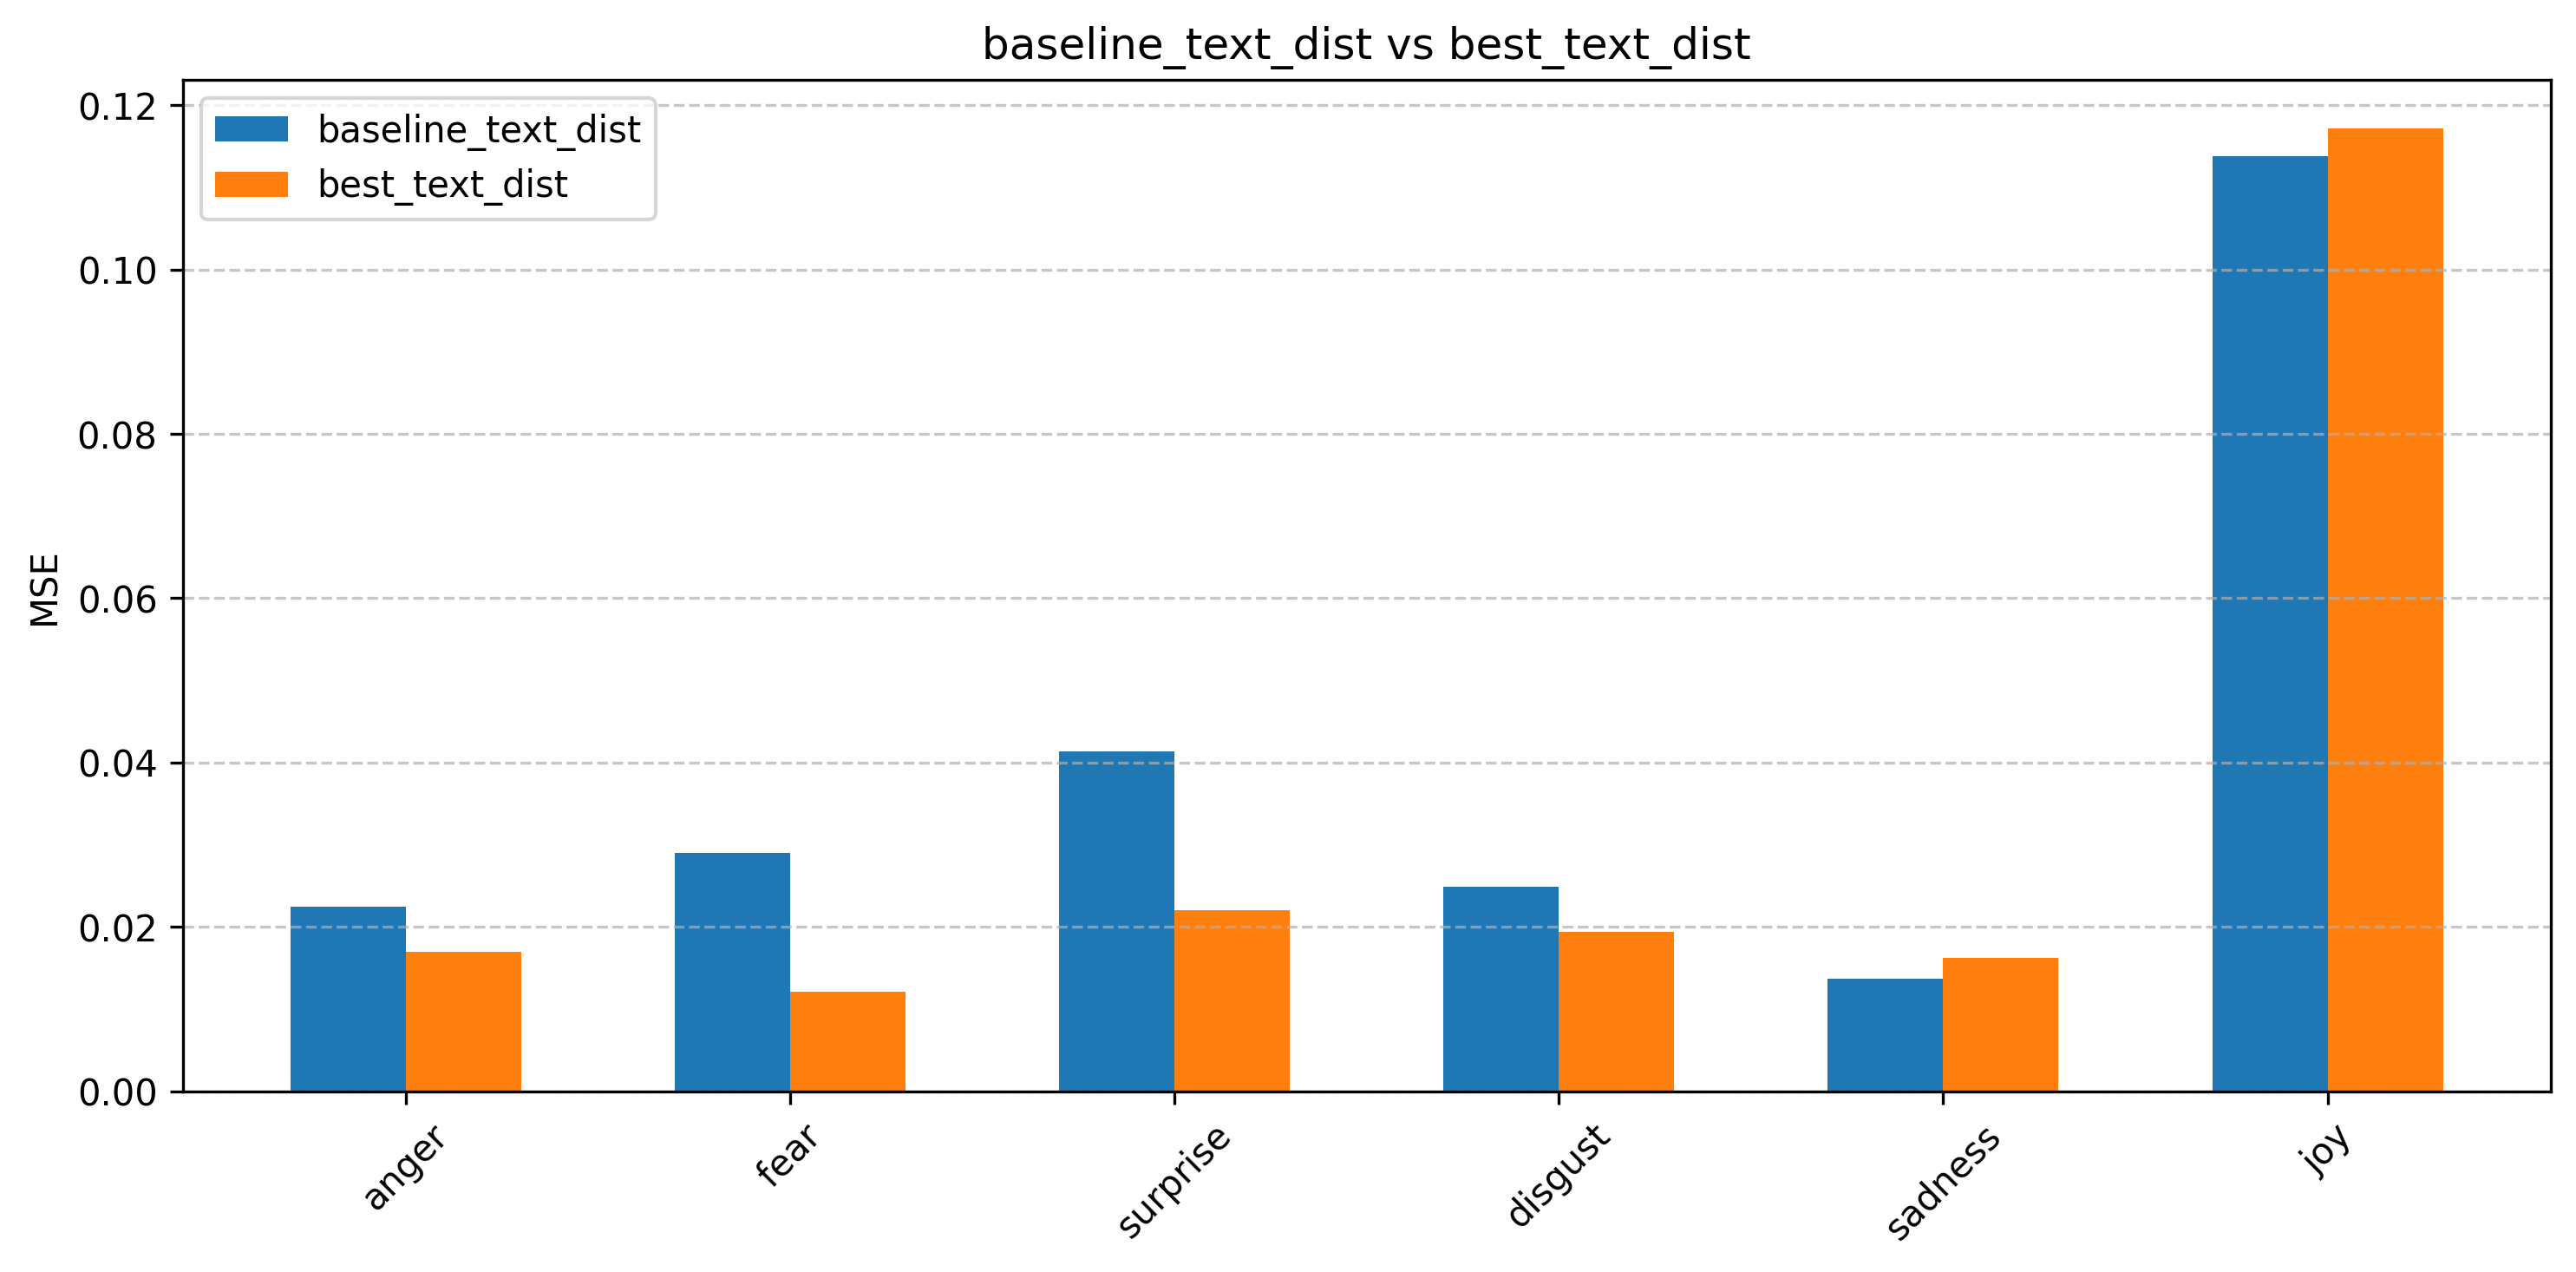
\includegraphics[width=\textwidth]{images/plot_1.png}
        \caption{MSE: Text model vs.\ baseline}
        \label{fig:mse-text}
    \end{subfigure}
    \hfill
    \begin{subfigure}[b]{0.48\textwidth}
        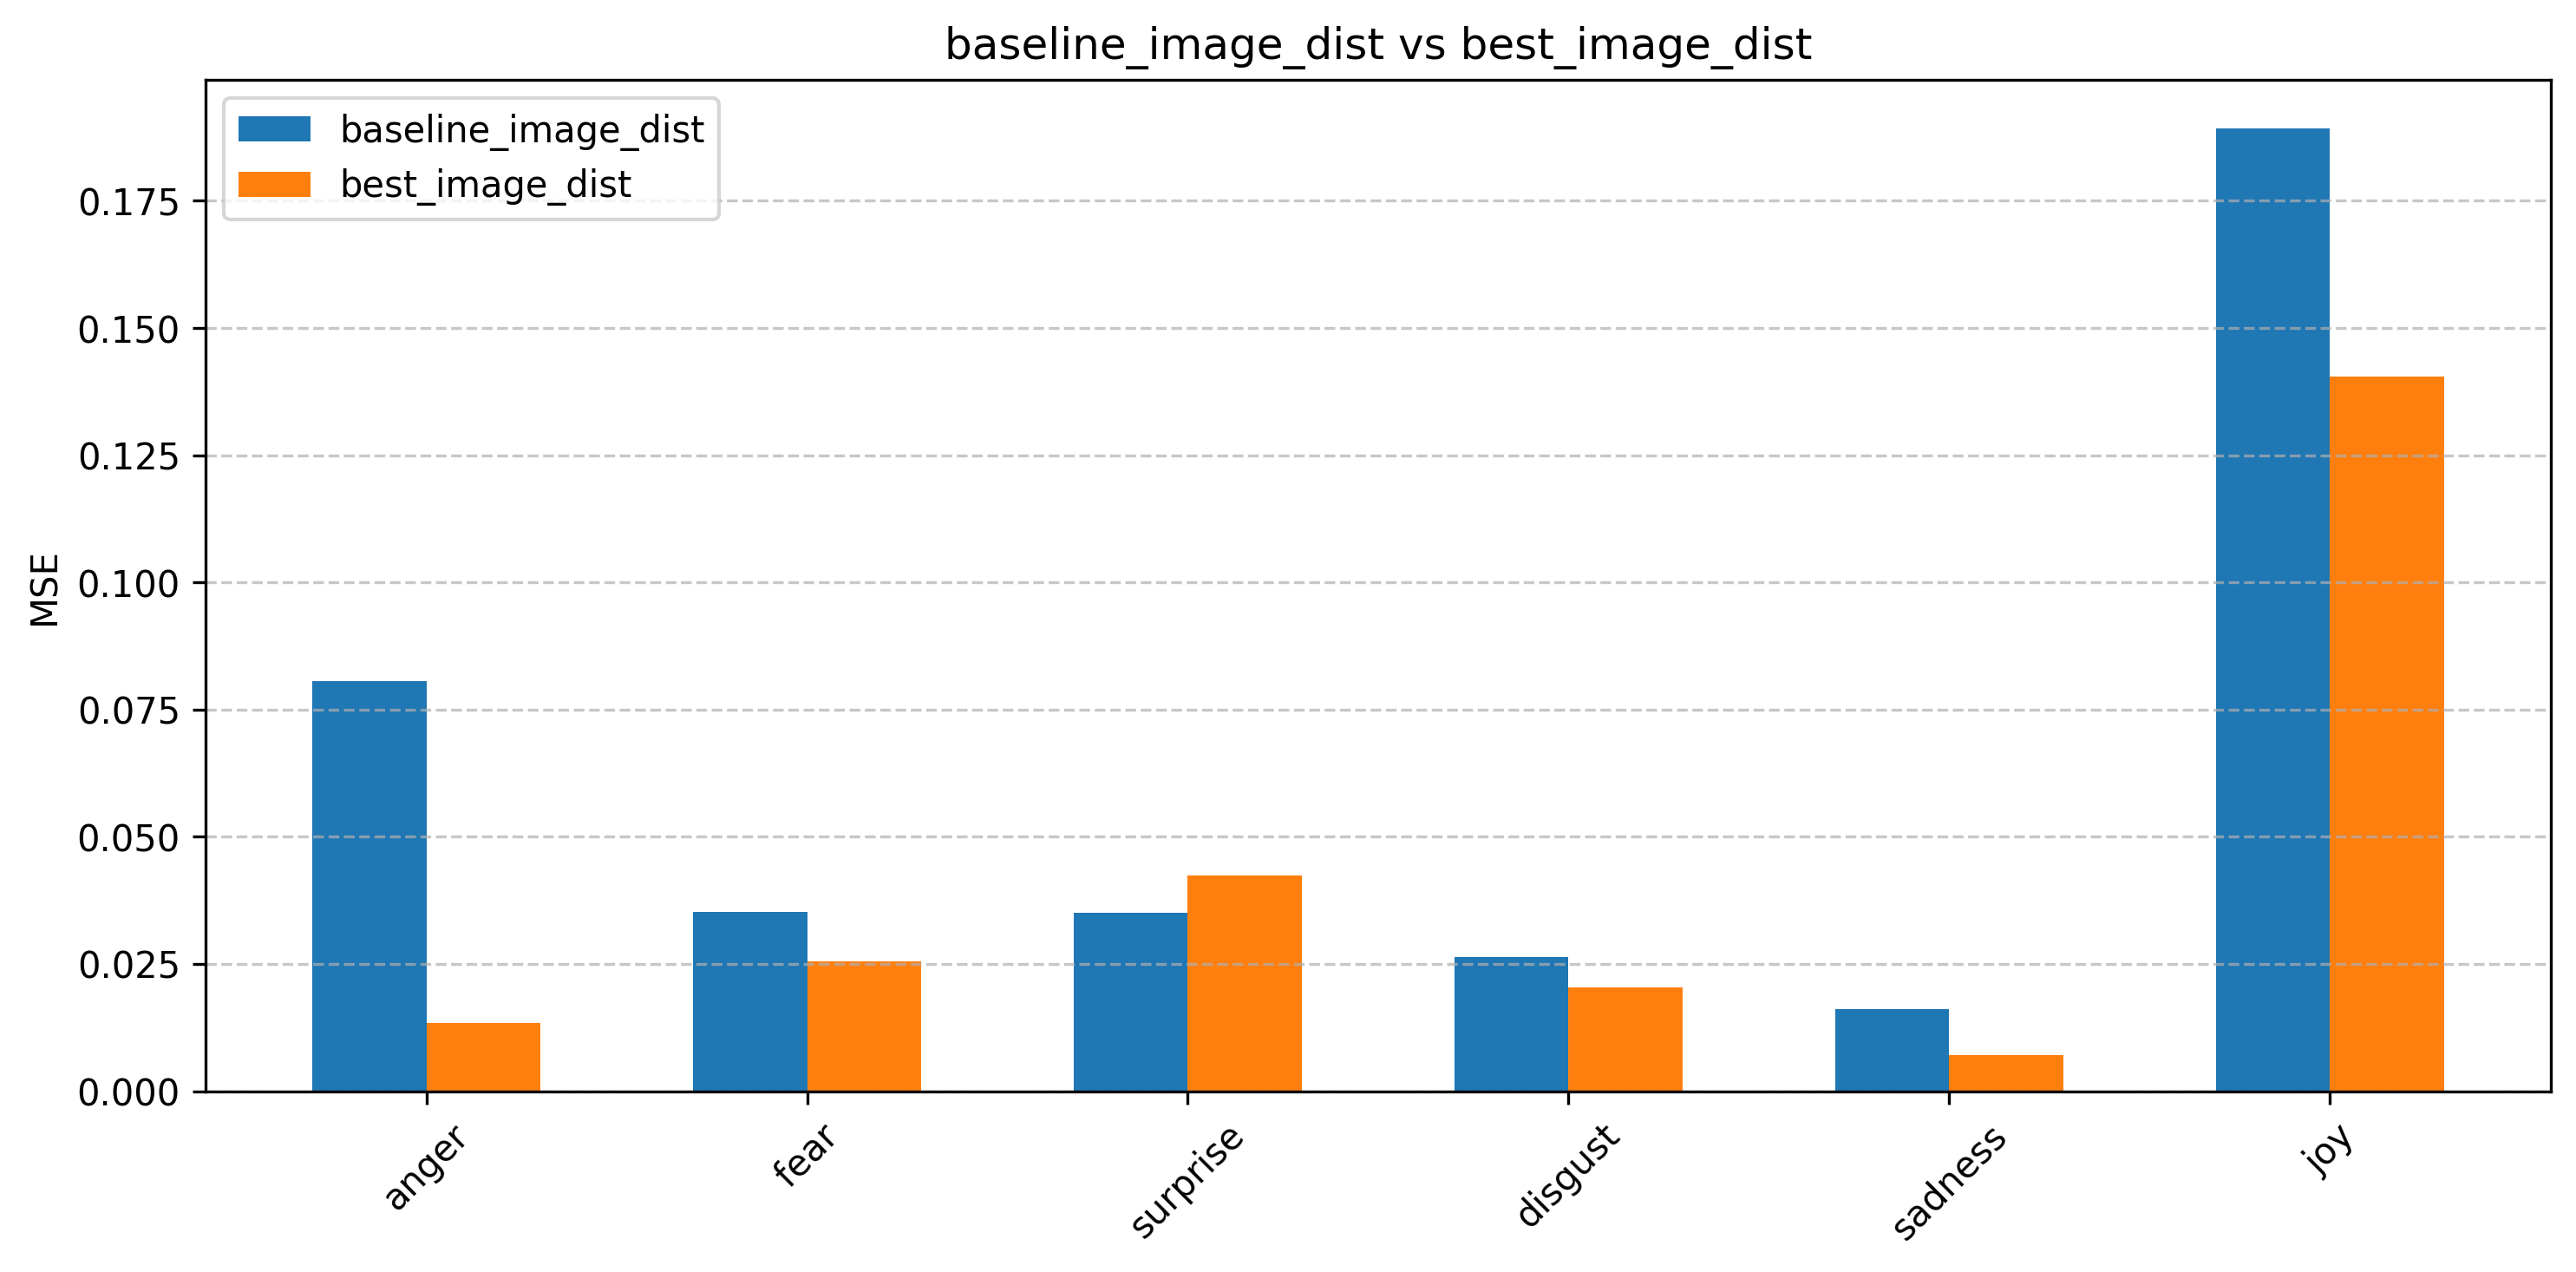
\includegraphics[width=\textwidth]{images/plot_2.png}
        \caption{MSE: Image model vs.\ baseline}
        \label{fig:mse-img}
    \end{subfigure}
    \begin{subfigure}[b]{0.48\textwidth}
        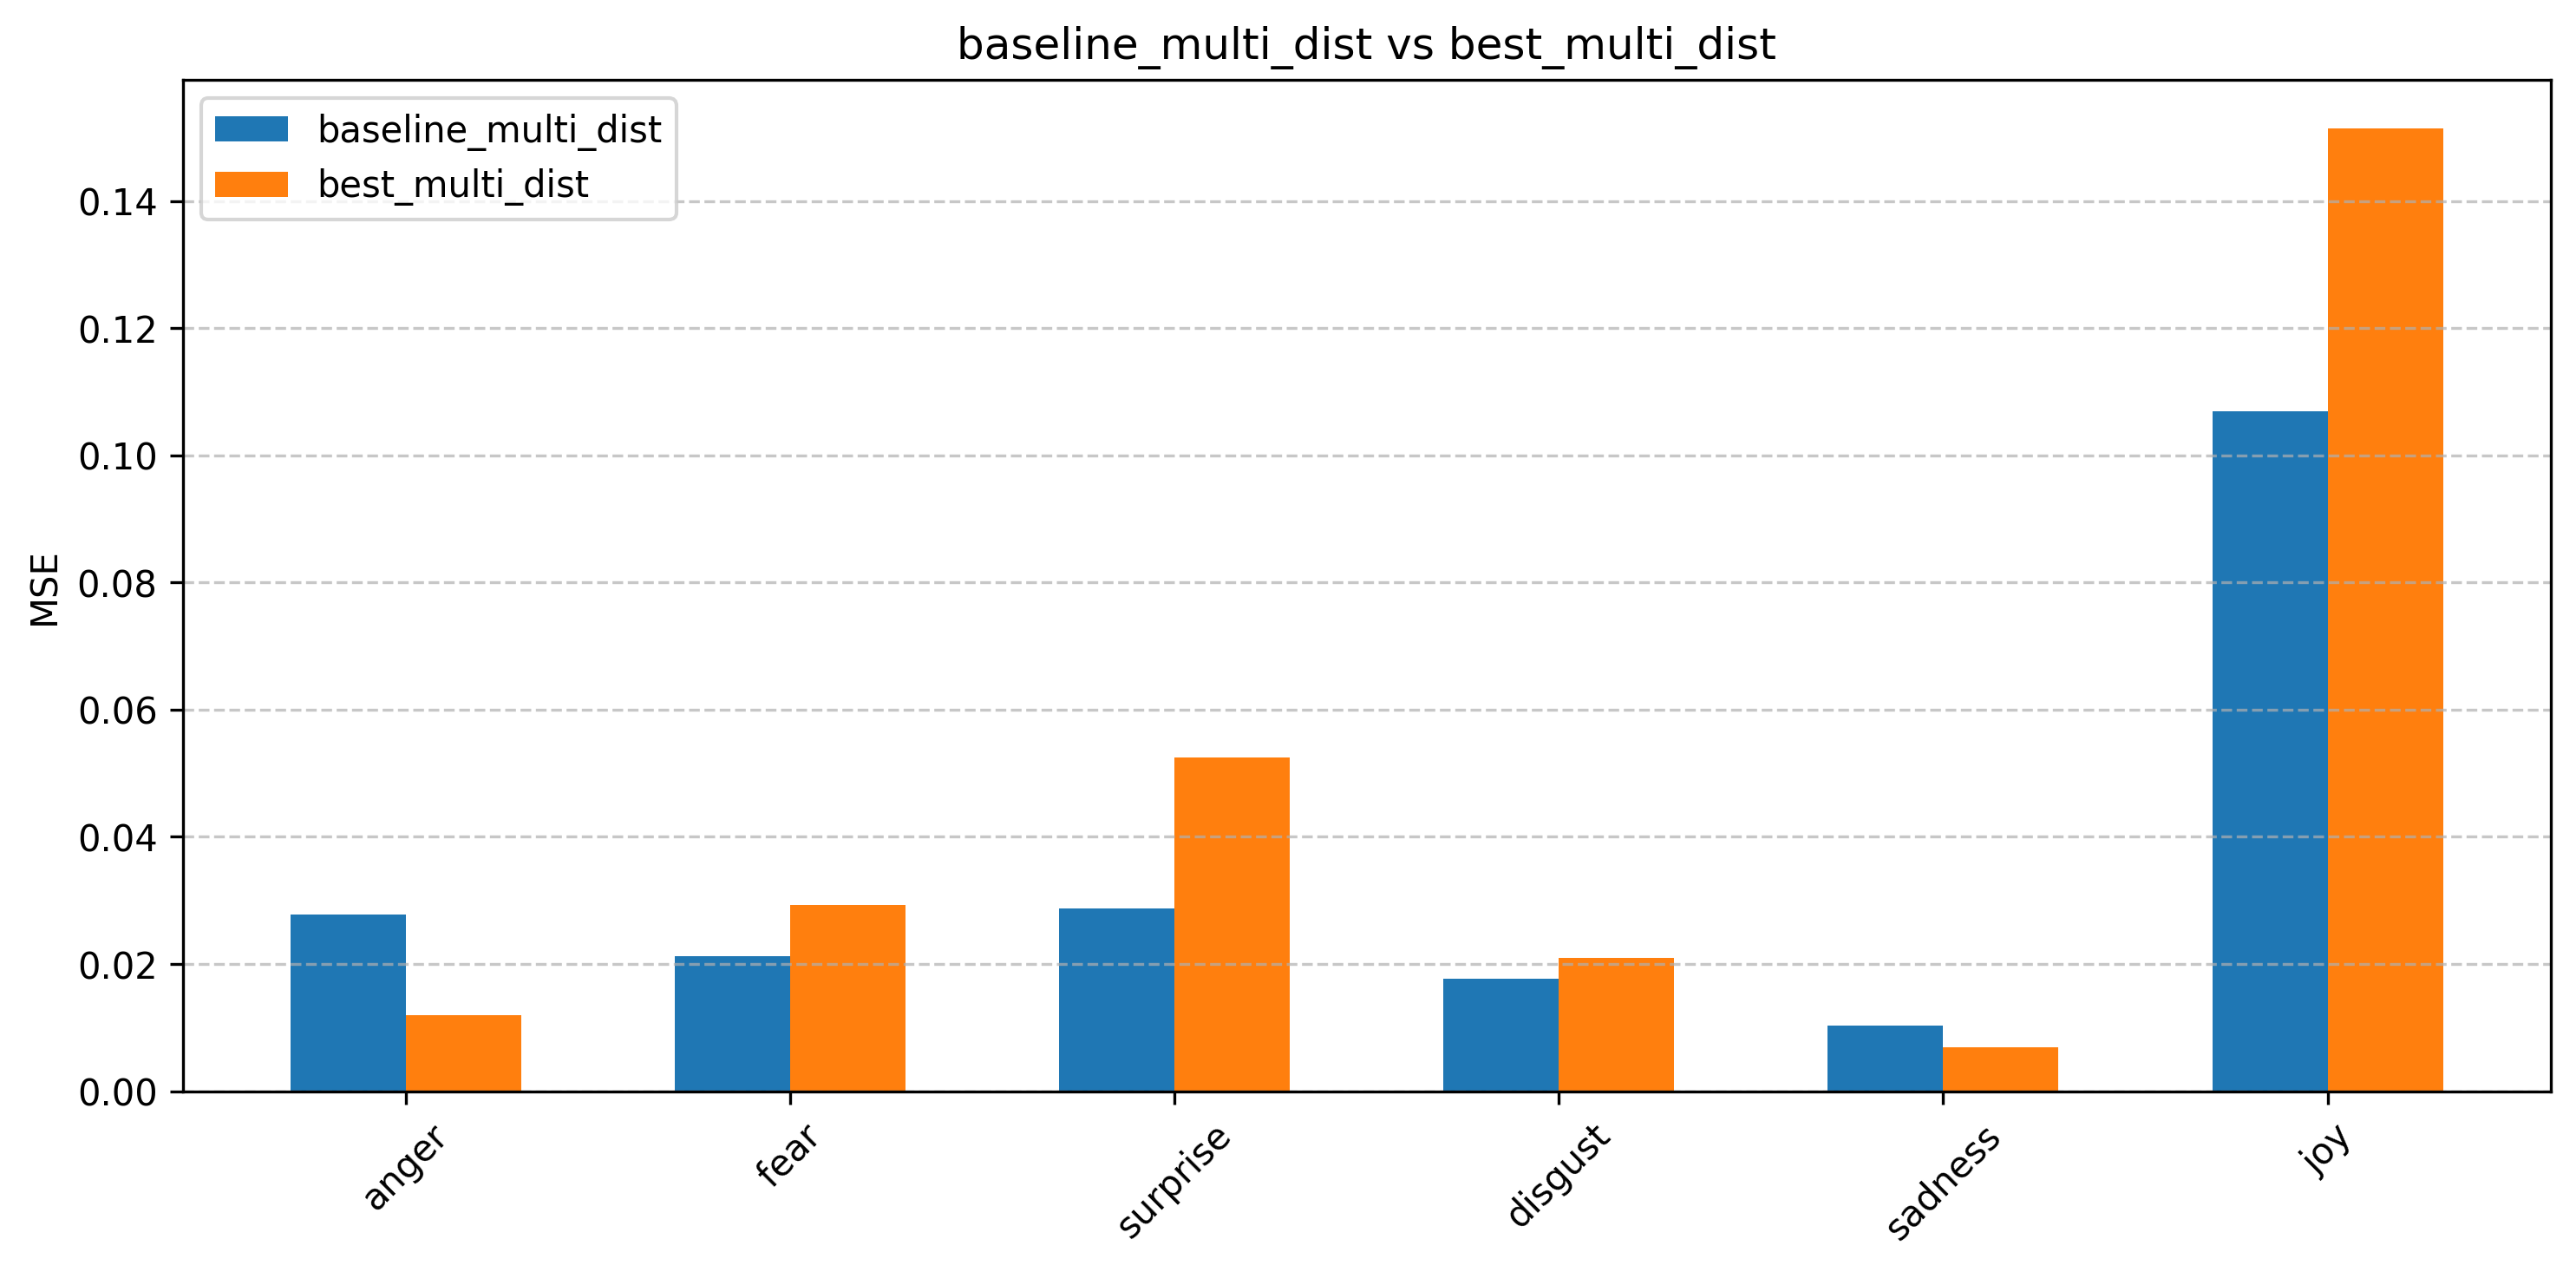
\includegraphics[width=\textwidth]{images/plot_3.png}
        \caption{MSE: Multimodal model vs.\ baseline}
        \label{fig:mse-multi}
    \end{subfigure}
    \caption{Emotion-wise comparison of Mean Squared Error (MSE) across models and baselines. Emotion order - Anger, Fear, Surprise, Disgust, Sadness, Joy. Lower is better.}
    \label{fig:mse-all}
\end{figure}

Despite significant gains in distribution metrics (Tables~\ref{tab:comparison}--\ref{tab:comparison_multi}), our models (text-only, image-only, and multimodal) still struggle with several recurring error patterns. We classify these issues into three main categories in subsections~\ref{subsec:cross-modal}--\ref{subsec:class-level}.

\begin{figure}[h]
    \centering
    \begin{subfigure}[b]{0.48\textwidth}
        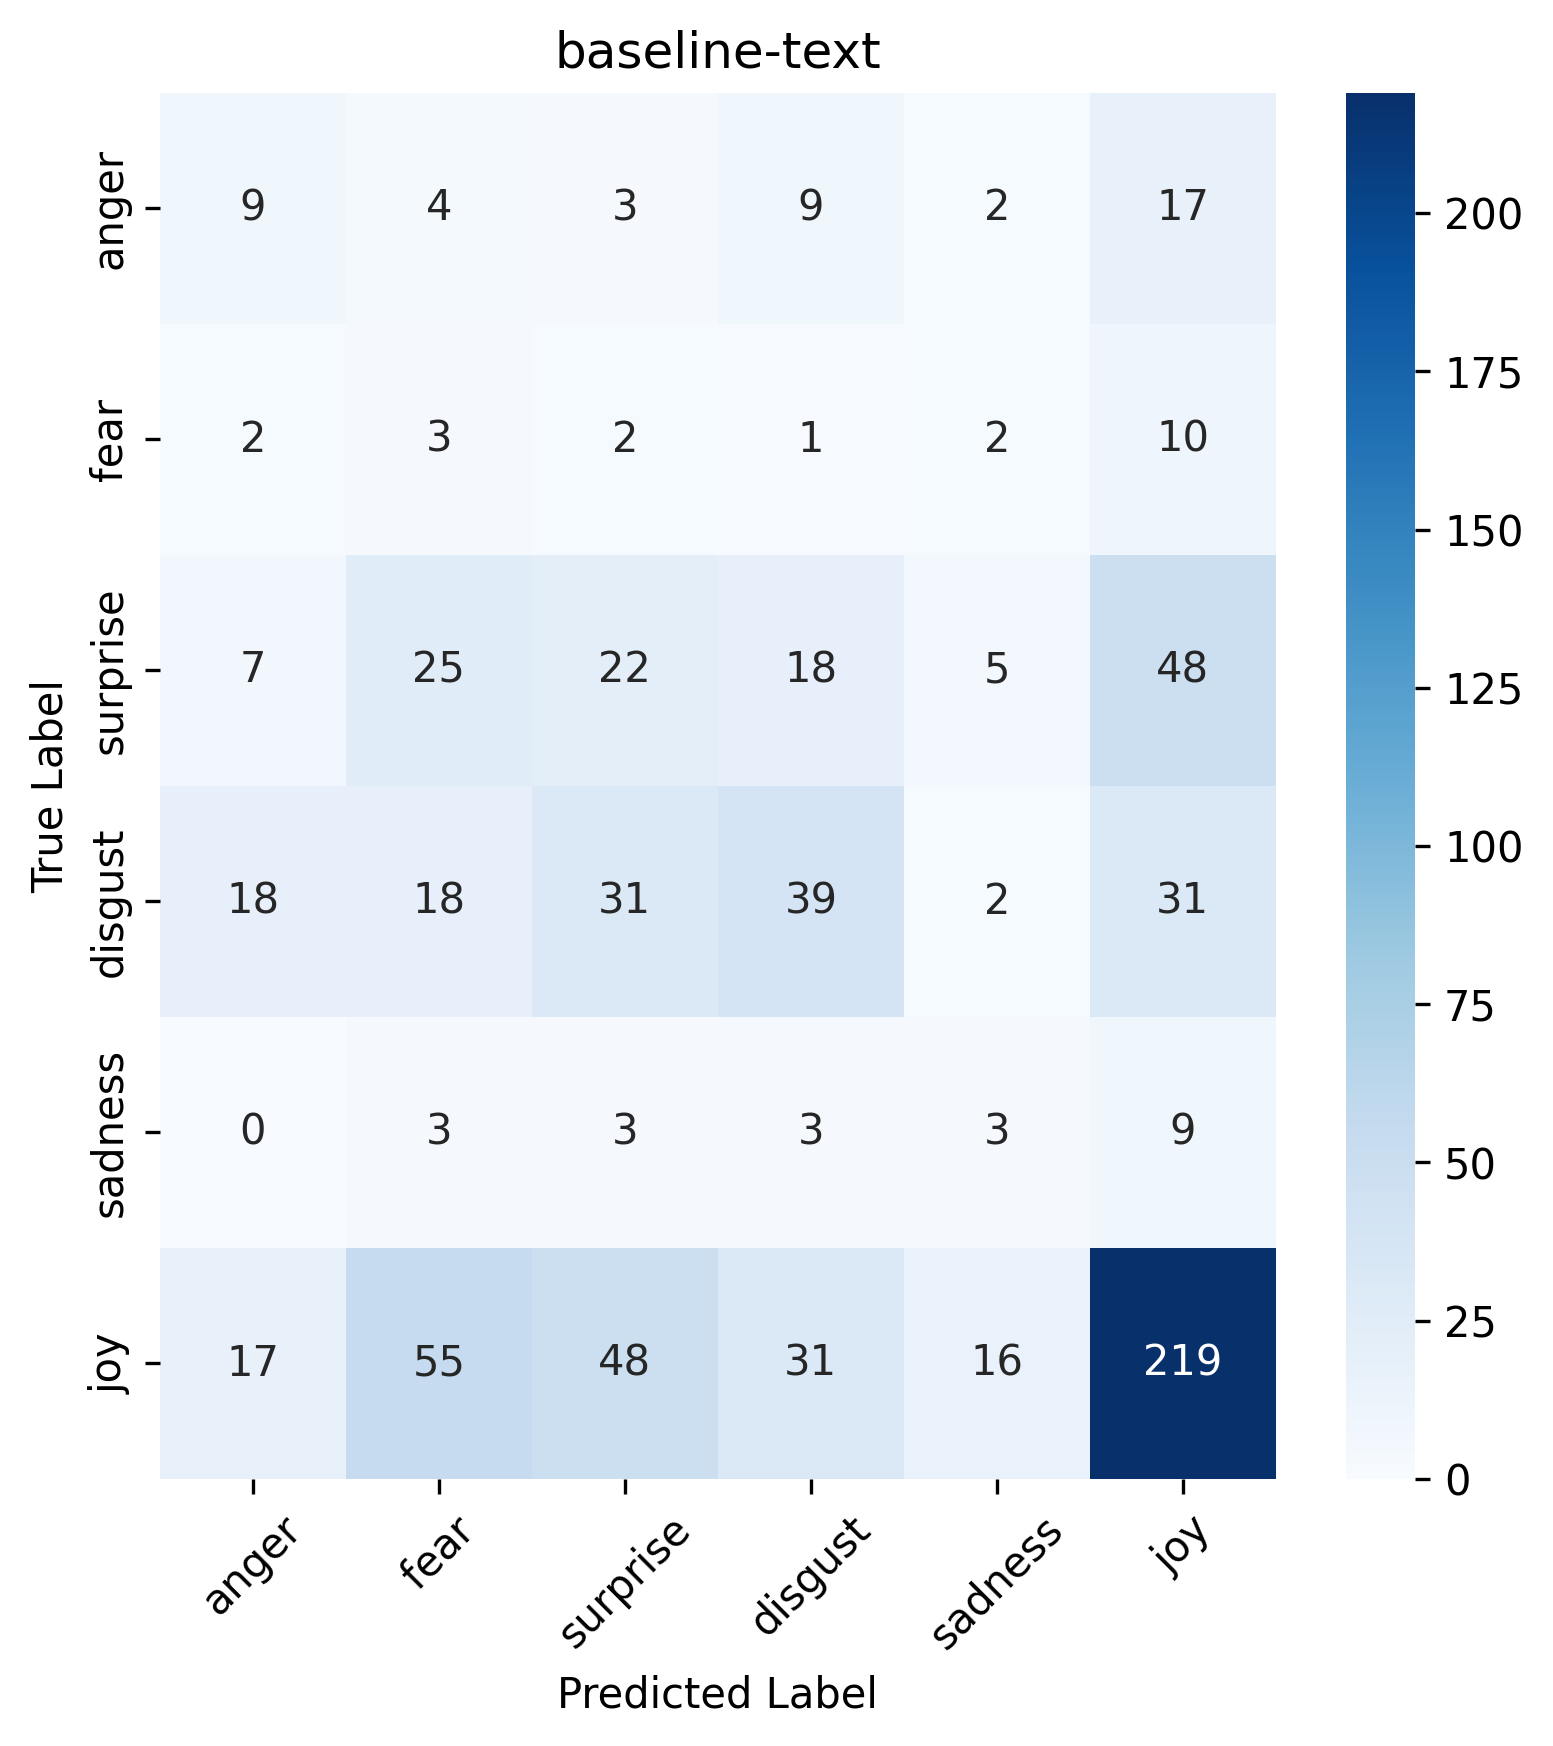
\includegraphics[width=\textwidth]{images/confusion_matrix_baseline_text_dist.png}
        \caption{Baseline Text Model.}
        \label{fig:text-confusion-baseline}
    \end{subfigure}
    \hfill
    \begin{subfigure}[b]{0.48\textwidth}
        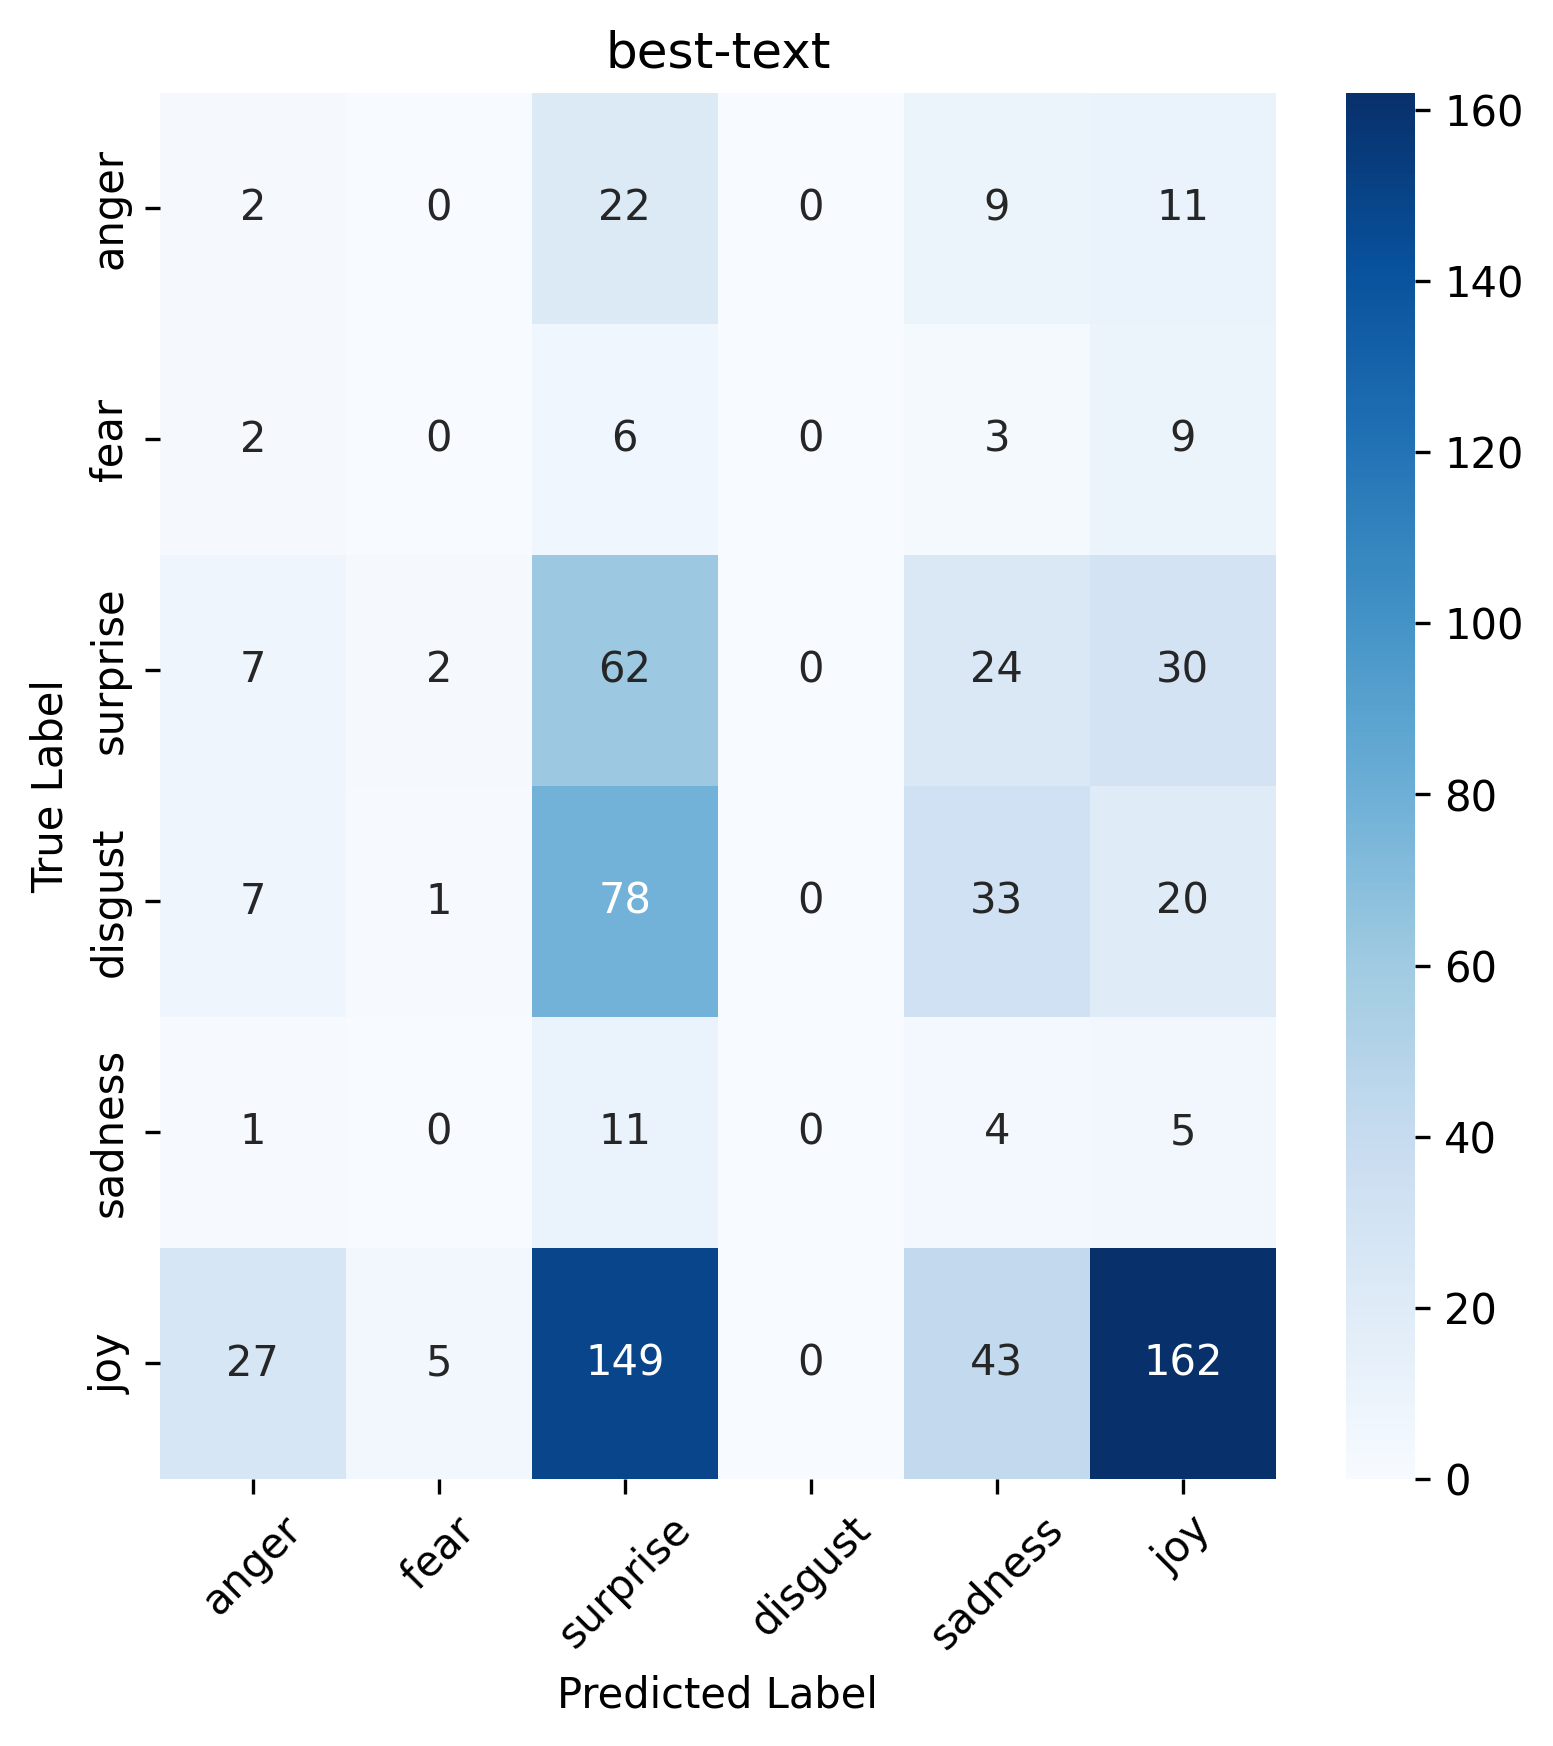
\includegraphics[width=\textwidth]{images/confusion_matrix_best_text_dist.png}
        \caption{Best Text Model.}
        \label{fig:text-confusion-best}
    \end{subfigure}
    \caption{Confusion matrices for text models. Darker blues indicate higher prediction frequency.}
    \label{fig:text-confusion}
\end{figure}

\begin{figure}[h]
    \centering
    \begin{subfigure}[b]{0.48\textwidth}
        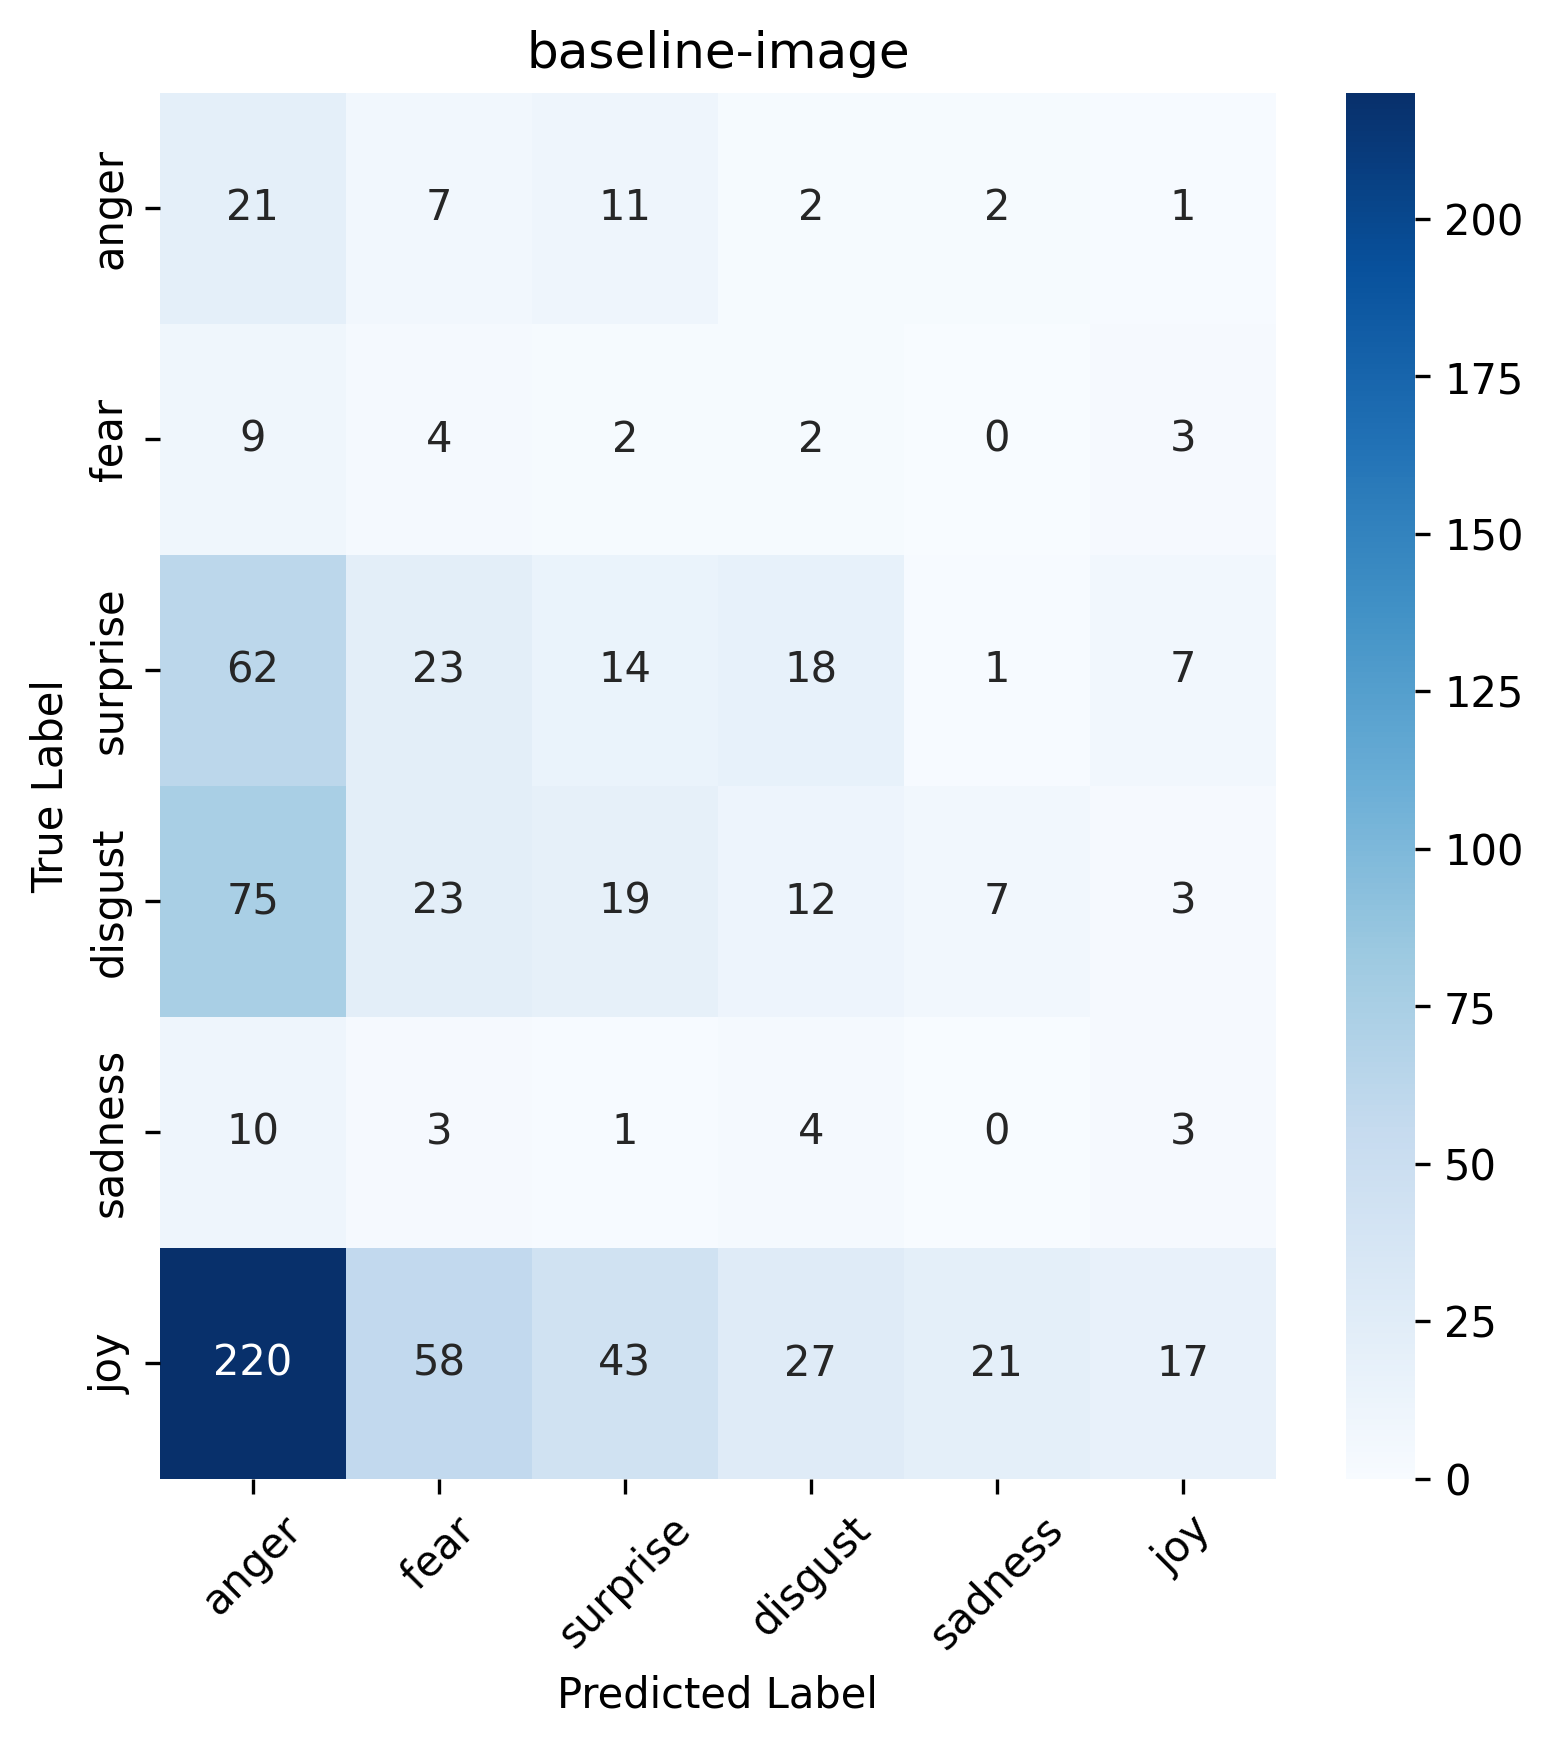
\includegraphics[width=\textwidth]{images/confusion_matrix_baseline_image_dist.png}
        \caption{Baseline Image Model.}
        \label{fig:image-confusion-baseline}
    \end{subfigure}
    \hfill
    \begin{subfigure}[b]{0.48\textwidth}
        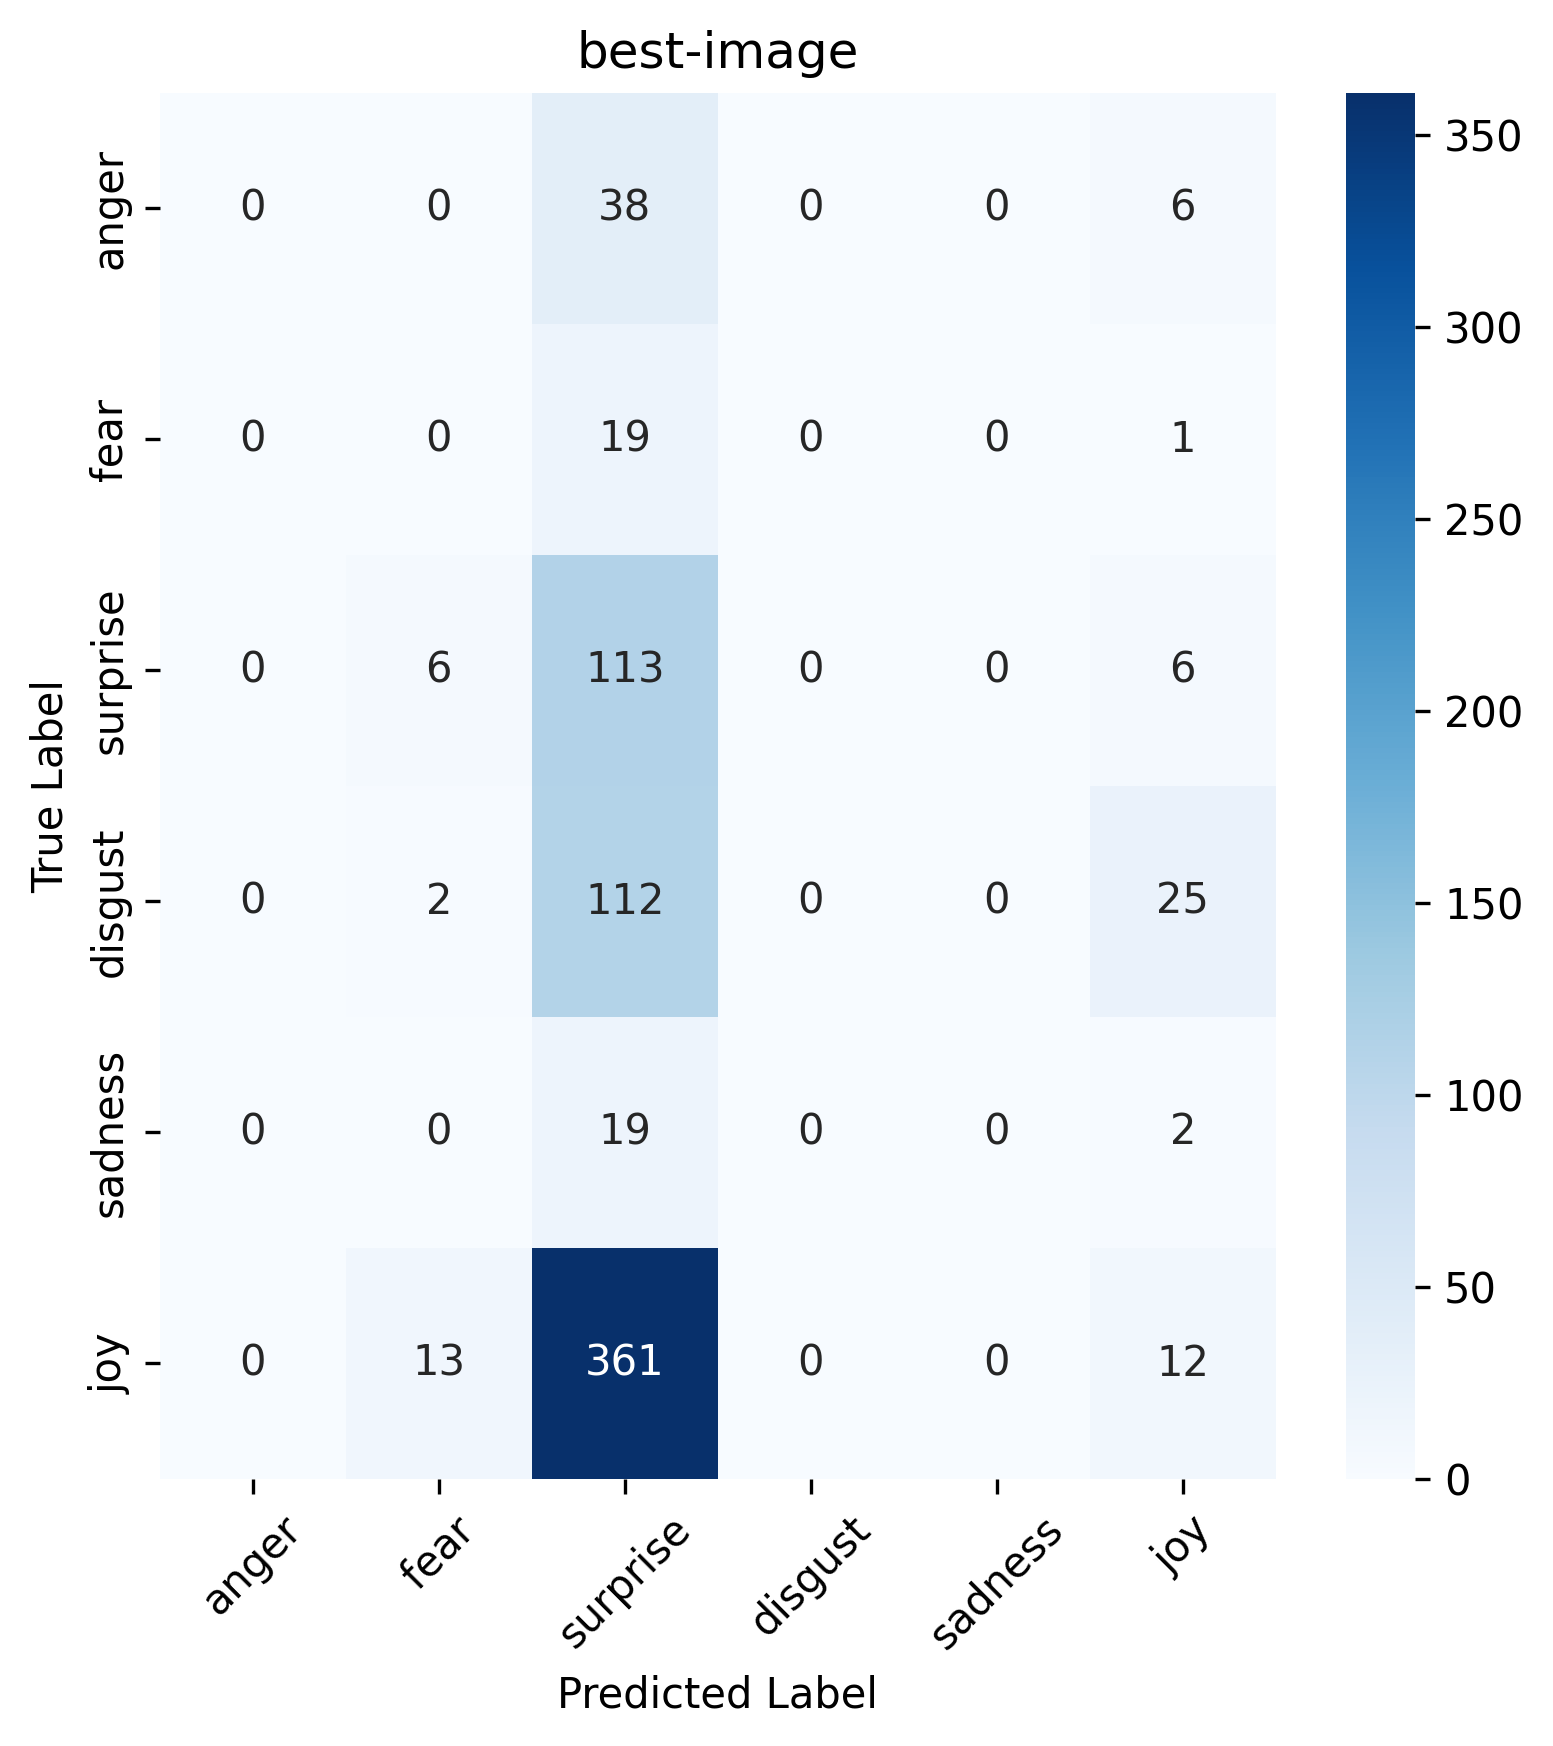
\includegraphics[width=\textwidth]{images/confusion_matrix_best_image_dist.png}
        \caption{Best Image Model.}
        \label{fig:image-confusion-best}
    \end{subfigure}
    \caption{Confusion matrices for image-only models.}
    \label{fig:image-confusion}
\end{figure}

\begin{figure}[h]
    \centering
    \begin{subfigure}[b]{0.48\textwidth}
        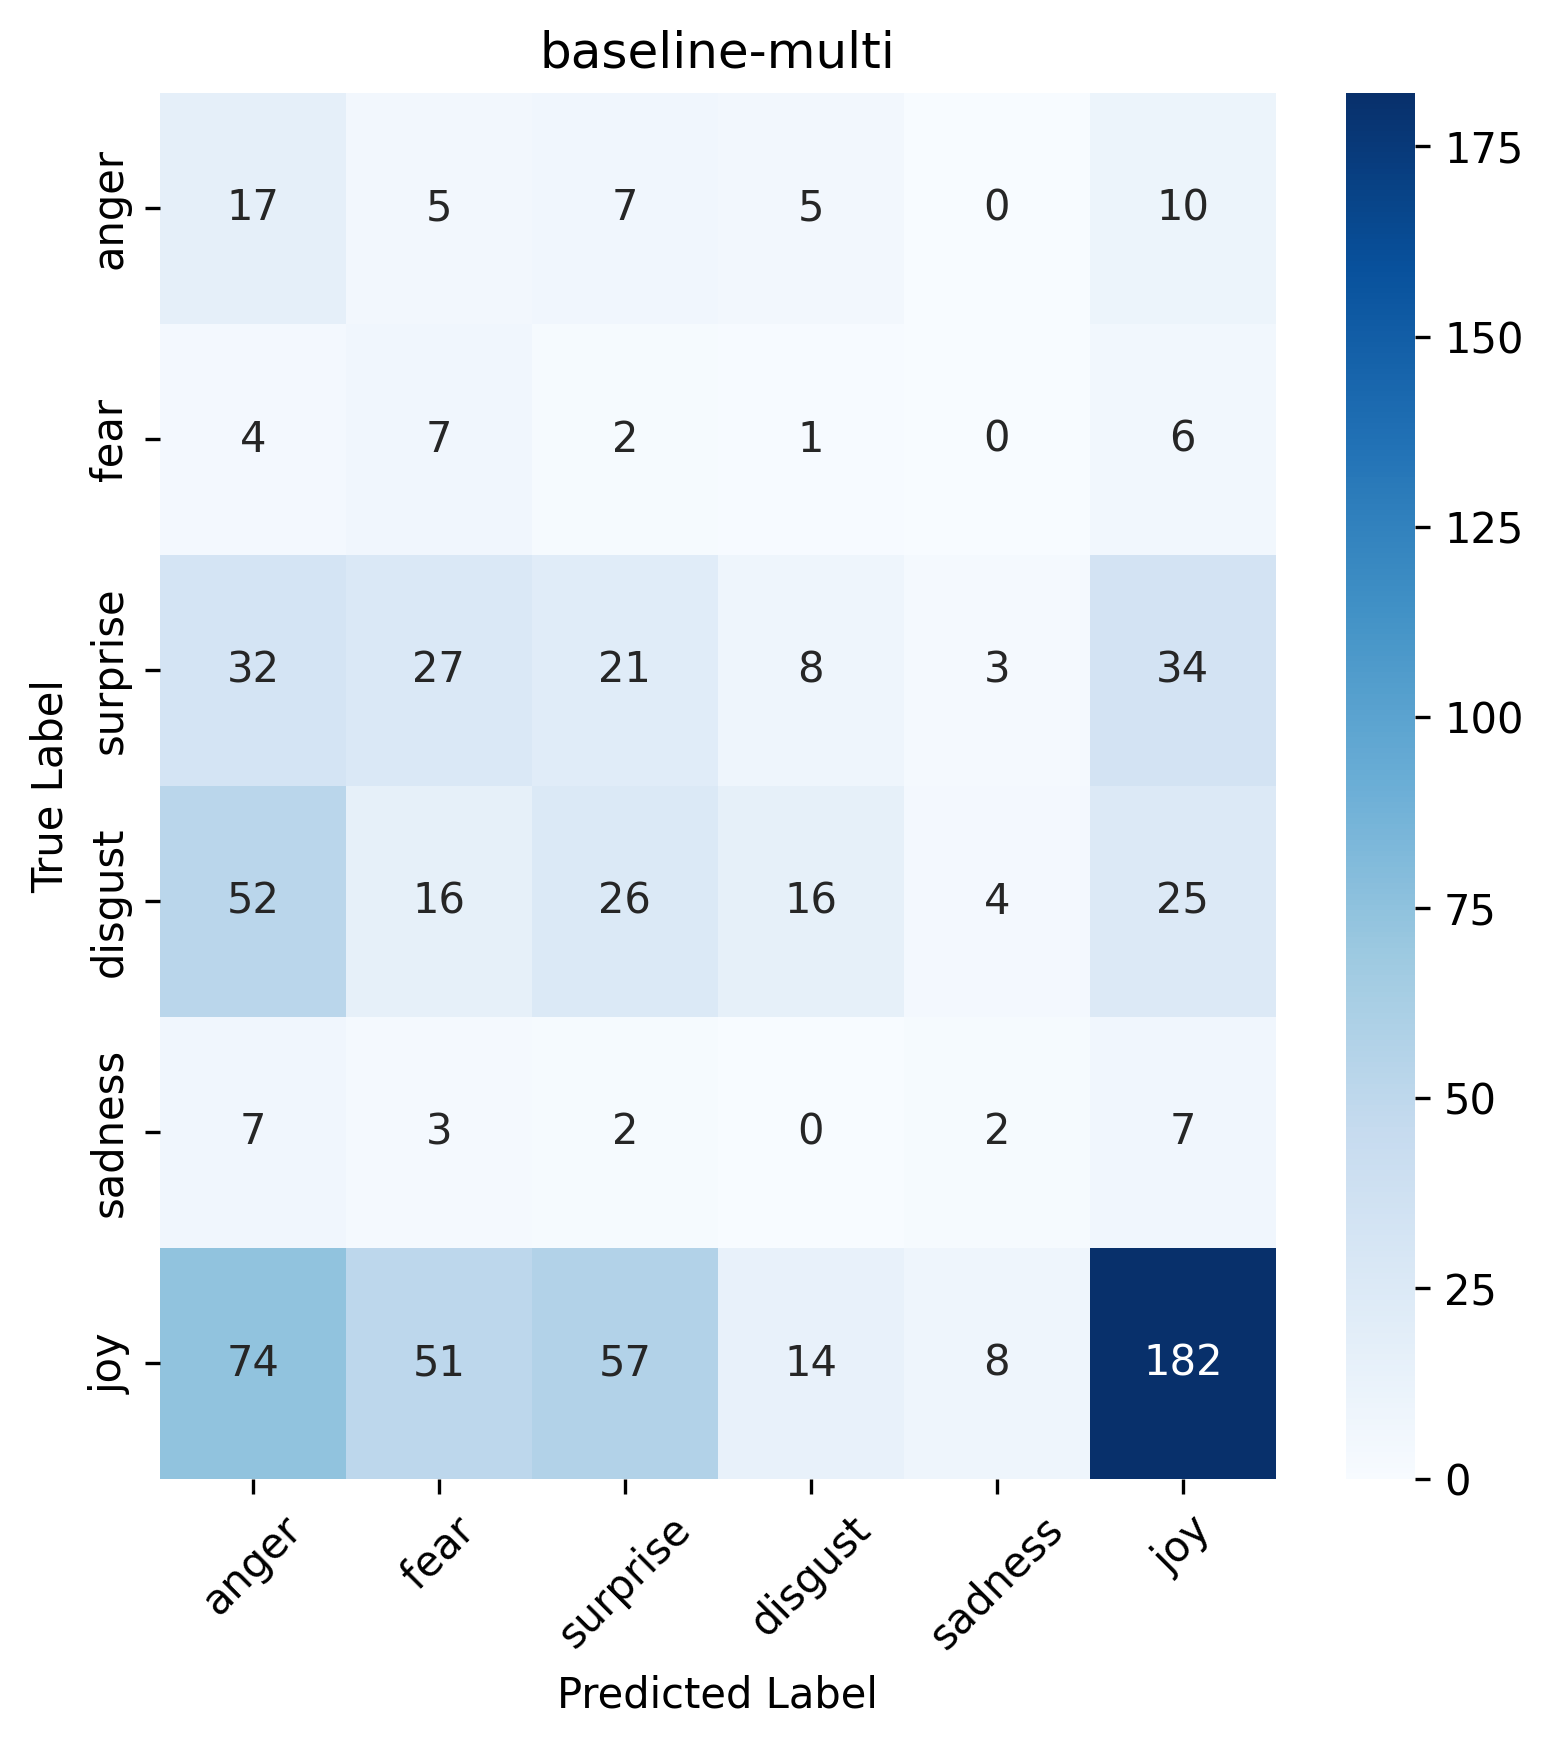
\includegraphics[width=\textwidth]{images/confusion_matrix_baseline_multi_dist.png}
        \caption{Baseline Multimodal.}
        \label{fig:multi-confusion-baseline}
    \end{subfigure}
    \hfill
    \begin{subfigure}[b]{0.48\textwidth}
        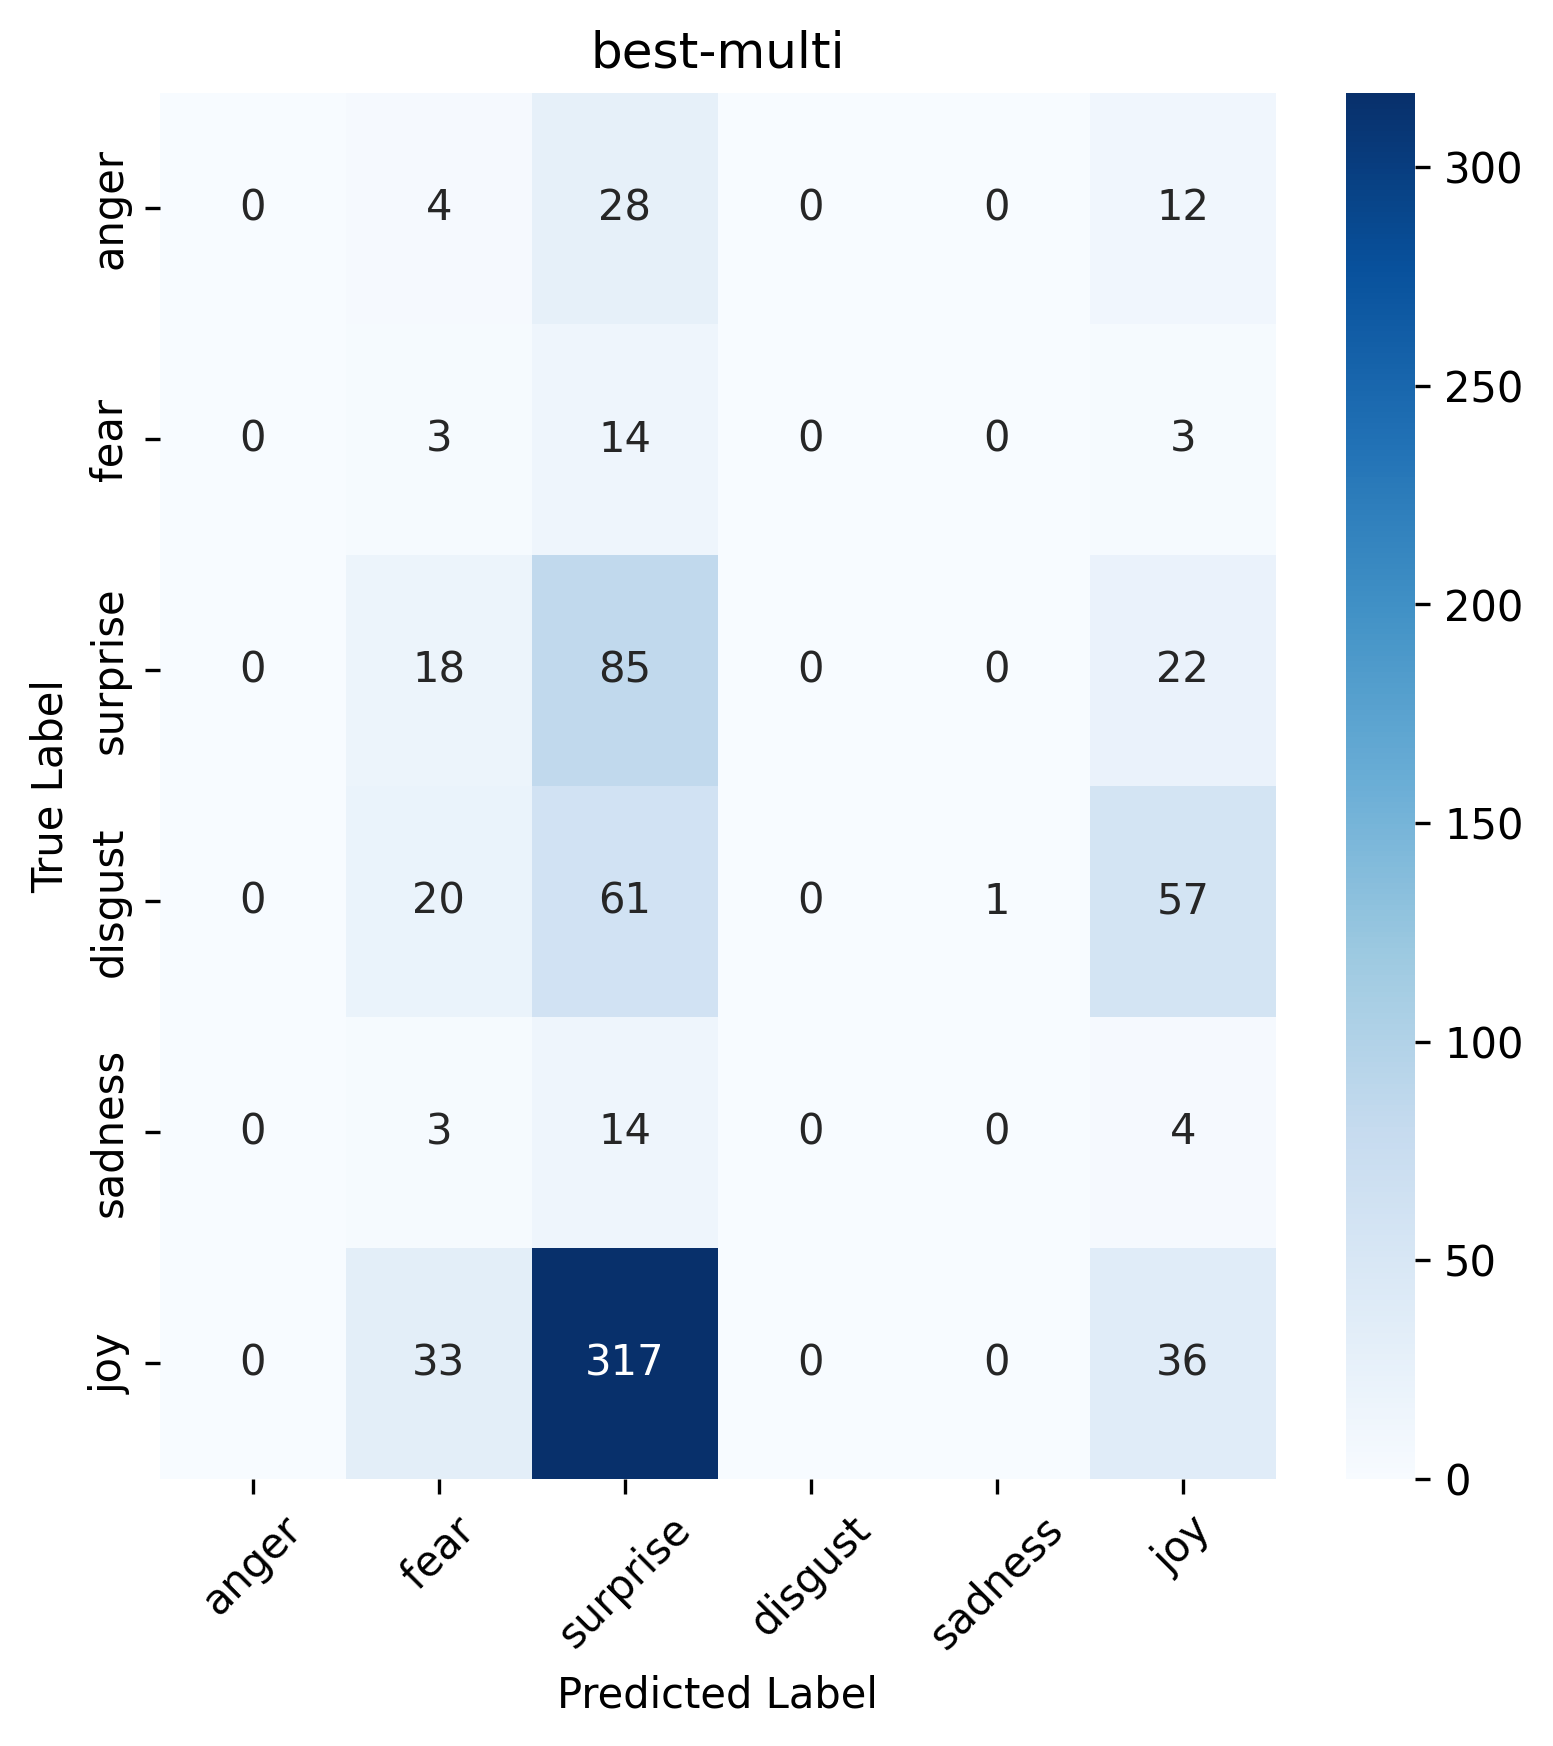
\includegraphics[width=\textwidth]{images/confusion_matrix_best_multi_dist.png}
        \caption{Best Multimodal.}
        \label{fig:multi-confusion-best}
    \end{subfigure}
    \caption{Multimodal confusion matrices.}
    \label{fig:multi-confusion}
\end{figure}

\subsection{Cross-Modal Error Patterns}
\label{subsec:cross-modal}

Our experiments reveal three broad error trends shared across text, image, and multimodal models:

\begin{itemize}
    \item \textbf{Minority Class Collapse.} Rare emotions such as \emph{sadness} or \emph{fear} remain poorly recognized, with recall often below 15\%. Text models frequently confuse \emph{sadness} with \emph{surprise} or \emph{joy} (79\% of errors), while image models can fail to detect \emph{sadness} altogether (0\% recall). Even though Mean Squared Error (MSE) drops by 35--64\% for some rare classes, Figure~\ref{fig:mse-all} and the confusion matrices confirm these mistakes persist.

    \item \textbf{Modality-Specific Overfitting.} Optimizing for distribution metrics can harm instance-level accuracy. Text-based models “forget” \emph{anger} (only 2 out of 44 correct) when improving other metrics. Image-only models overcompensate for \emph{anger} bias, predicting \emph{surprise} almost exclusively (113/125 correct on \emph{surprise}, but 361 false positives). Multimodal fusion inherits both problems, absorbing the text model's \emph{sadness} mistakes (92\% misclassifications) and the image model's \emph{surprise} bias.

    \item \textbf{Distribution-Instance Dissonance.} Large gains in cosine similarity (16--56\% improvement) can mask argmax errors. For example, \emph{joy} appears best predicted (162--219 correct in text models), but this partly stems from excessive \emph{joy} predictions (36--48\% of all outputs). The inherent trade-off between distributional alignment and per-instance fidelity remains a core challenge.
\end{itemize}


\subsection{Class-Level Analysis}
\label{subsec:class-level}

To better understand model misclassifications, we closely examine both the confusion matrices (Figures~\ref{fig:text-confusion}--\ref{fig:multi-confusion}) and the MSE trends (Figure~\ref{fig:mse-all}; also see the per-class MSE values in Tables~\ref{tab:comparison}--\ref{tab:comparison_multi}).

\paragraph{Text Model.} 
From Table~\ref{tab:comparison}, the \emph{best text model} achieves notable MSE reductions for \emph{anger} (0.0224$\rightarrow$0.0170) and \emph{fear} (0.0290$\rightarrow$0.0121) compared to the baseline. However, it slightly increases MSE for \emph{sadness} (0.0137$\rightarrow$0.0162) and \emph{joy} (0.1138$\rightarrow$0.1172). This trade-off is also reflected in Figure~\ref{fig:text-confusion-best} (row 5: sadness), where only 3 of 18 sadness instances are correctly identified. The confusion matrix further reveals that \emph{anger} is often misclassified as \emph{surprise} (22 out of 44 anger instances).

\paragraph{Image Model.} 
For image-only models (Table~\ref{tab:comparison}), the \emph{best image model} significantly lowers MSE for \emph{joy} (0.1892$\rightarrow$0.1405) but worsens for \emph{surprise} (0.0350$\rightarrow$0.0424). In Figure~\ref{fig:image-confusion-best}, the majority of misclassifications (361 false positives) come from mistakenly predicting \emph{surprise}, which also damages \emph{disgust} recognition (79\% mislabeled as \emph{surprise}). Hence, while distribution metrics improve overall, the confusion matrix illustrates a strong one-label bias.

\paragraph{Multimodal Model.}
Finally, the multimodal model (Table~\ref{tab:comparison_multi}) shows mixed gains. The \emph{best multimodal} run achieves lower MSE for \emph{anger} (0.0278$\rightarrow$0.0120) and \emph{sadness} (0.0103$\rightarrow$0.0069) but raises MSE for \emph{surprise} (0.0287$\rightarrow$0.0525) and \emph{joy} (0.1070$\rightarrow$0.1514). The confusion matrix in Figure~\ref{fig:multi-confusion-best} confirms that a large portion of \emph{disgust} entries (61\%) are absorbed into \emph{surprise}, indicating the model struggles to differentiate negative emotions when trained to optimize overall distribution resemblance. Freezing text layers (to retain gains on \emph{fear} and \emph{anger}) can, unfortunately, lock in earlier classification mistakes, such as \emph{sadness} $\rightarrow$ \emph{joy} mislabels.

\subsubsection{Findings}

\begin{itemize}
    \item \textbf{Improvements in Rare Classes Are Fragile.} While MSE for \emph{anger} and \emph{fear} generally decreases, confusion matrices reveal significant misclassifications into \emph{surprise} or \emph{joy}. Minor distribution changes can drastically alter these minority-class predictions.
    
    \item \textbf{Overproduction of Dominant Emotions.} In both the text and image models, \emph{surprise} and \emph{joy} are predicted too often (see darker cells in Figures~\ref{fig:text-confusion}--\ref{fig:image-confusion}). This skew helps match the global emotion distribution but harms per-instance accuracy.
    
    \item \textbf{Multimodal Fusion Conflicts.} Although combining text and image usually improves distribution metrics, the confusion matrices (Figures~\ref{fig:multi-confusion-best}) highlight how errors from each modality can reinforce each other rather than cancelling out. Notably, \emph{disgust} is frequently overridden by the image model’s \emph{surprise} bias, and \emph{sadness} from text is often lost to \emph{joy}.
\end{itemize}

In summary, while distribution-level metrics show progress, real-use scenarios require robust, per-instance predictions. Our analysis of the confusion matrices and MSE trends underscores the persistent difficulty in balancing minority-class accuracy with global distribution alignment. Addressing these issues will likely require new architectures and training strategies (e.g., multi-task losses, calibration techniques, or explicit rare-class focus) rather than pure metric optimization.





\section{Qualitative Analysis}

In this section, we present a detailed qualitative analysis of our emotion distribution predictions. Alongside each tweet snippet and its aggregated distribution of replies (the ``gold" target), we also show samples of \emph{individual} reply predictions. This provides insight into how each user response contributes to the final averaged (aggregated) target distribution and how the model might struggle or excel in capturing these varied emotional signals.

\vspace{1em}
\subsection*{Poor Performance Cases}

\begin{figure}[h]
    \centering
    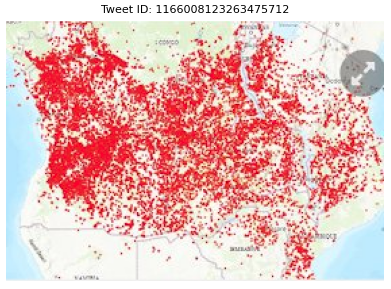
\includegraphics[width=0.4\textwidth]{images/bad1.png} 
    \hfill
    
\includegraphics[width=0.4\textwidth]{images/bad2.png}
    \caption{Examples of high-error predictions (Case A on left, Case B on right).}
    \label{fig:bad_cases}
\end{figure}

\subsubsection*{Case A: Tweet ID 1166008123263475712}

\noindent\textbf{Text Snippet:}
\begin{quote}
\#AlTenoorOverflow \#Africafires \#Angola \#Zambia \#Tanzania \#Congo \\
Links to the \#SkirmishEvents statements in multiple languages: [URLs]
\end{quote}

\noindent\textbf{Aggregated Reply Distribution (1 reply):}
\[
\begin{aligned}
\{\text{anger: } 0.0694, \quad \text{fear: } 0.4879, \quad \text{surprise: } 0.0686, \\
\text{disgust: } 0.0421, \quad \text{sadness: } 0.3046, \quad \text{joy: } 0.0274\}
\end{aligned}
\]

\noindent\textbf{Our Predictions (Text-only):}
\[
\begin{aligned}
\{\text{anger: } 0.1701, \quad \text{fear: } 0.1532, \quad \text{surprise: } 0.2239, \\
\text{disgust: } 0.1151, \quad \text{sadness: } 0.1629, \quad \text{joy: } 0.1749\}
\end{aligned}
\]

\noindent\textbf{Our Predictions (Image-only):}
\[
\begin{aligned}
\{\text{anger: } 0.1181, \quad \text{fear: } 0.2317, \quad \text{surprise: } 0.2666, \\
\text{disgust: } 0.1130, \quad \text{sadness: } 0.1180, \quad \text{joy: } 0.1526\}
\end{aligned}
\]

\noindent\textbf{Our Predictions (Multimodal):}
\[
\begin{aligned}
\{\text{anger: } 0.1089, \quad \text{fear: } 0.2705, \quad \text{surprise: } 0.2549, \\
\text{disgust: } 0.0992, \quad \text{sadness: } 0.1060, \quad \text{joy: } 0.1606\}
\end{aligned}
\]

Since only one user replied, the aggregated distribution essentially mirrors that single reply’s predicted emotions. The user’s response shows a dominant signal of \emph{fear} and \emph{sadness}:

\begin{quote}
\emph{``Enlightenment at a time when the world began to turn towards fires, 
it turns out that fires broke out in entire countries in sub-Saharan Africa...''}
\end{quote}

Despite this clear emotional focus (with nearly half the probability mass on \textit{fear}), the model’s final (multimodal) prediction spread its probabilities more evenly, assigning:

\begin{itemize}
    \item \textit{Fear:} 27.0\% (vs.\ 48.8\% in replies),
    \item \textit{Sadness:} 18.3\% (vs.\ 30.5\%),
    \item Extra probability mass on \textit{Anger} and \textit{Surprise}.
\end{itemize}

Notably, the text-only predictions (\textit{fear}: 15.3\%, \textit{sadness}: 16.3\%) and image-only predictions (\textit{fear}: 23.2\%, \textit{sadness}: 11.8\%) also dispersed their probability across other emotions like \textit{anger} and \textit{surprise}, failing to capture the strong peaks in \textit{fear} and \textit{sadness}. While the image-only model gave a slightly higher estimate for \textit{fear} (23.2\%), it still significantly underestimated both top emotions relative to the aggregated reply.
\newline

This mismatch highlights how \textbf{low-entropy replies} (favouring one or two emotions) can lead to larger KL divergence when the model avoids placing too much confidence in a single label. Our KL-based training objective often prevents the model from collapsing onto a single dominant peak—resulting in a more ``flattened” (high-entropy) prediction distribution.

\subsubsection*{Case B: Tweet ID 1161715780523896832}

\noindent\textbf{Text Snippet:}
\begin{quote}
[USER] set sail today (sailboat) so..who’s in to \#StrikeWithUs (fire)(earth)? (world map) \\
\textbf{Find Your Local Event} [URL] \quad
\textbf{Search Climate Actions} [URL] \quad
\textbf{Organize \& Promote Your Own} [URL] \\
GO (raised fist)(raised fist)(raised fist)(raised fist) \#Fridays4Future [URL]
\end{quote}

\noindent\textbf{Aggregated Reply Distribution (1 reply):}
\[
\begin{aligned}
\{\text{anger: } 0.0498, \quad \text{fear: } 0.0740, \quad \text{surprise: } 0.6239, \\
\text{disgust: } 0.0973, \quad \text{sadness: } 0.0866, \quad \text{joy: } 0.0683\}
\end{aligned}
\]

\noindent\textbf{Our Predictions (Text-only):}
\[
\begin{aligned}
\{\text{anger: } 0.1408, \quad \text{fear: } 0.1396, \quad \text{surprise: } 0.2146, \\
\text{disgust: } 0.1536, \quad \text{sadness: } 0.1299, \quad \text{joy: } 0.2212\}
\end{aligned}
\]

\noindent\textbf{Our Predictions (Image-only):}
\[
\begin{aligned}
\{\text{anger: } 0.1063, \quad \text{fear: } 0.2226, \quad \text{surprise: } 0.3884, \\
\text{disgust: } 0.0765, \quad \text{sadness: } 0.0701, \quad \text{joy: } 0.1359\}
\end{aligned}
\]

\noindent\textbf{Our Predictions (Multimodal):}
\[
\begin{aligned}
\{\text{anger: } 0.0844, \quad \text{fear: } 0.2314, \quad \text{surprise: } 0.4655, \\
\text{disgust: } 0.0664, \quad \text{sadness: } 0.0569, \quad \text{joy: } 0.0954\}
\end{aligned}
\]

There was only a single reply, predominantly expressing \textbf{surprise (62.4\%)}. The user’s short reaction suggests excitement or astonishment regarding the climate strike:
\begin{quote}
\emph{``p.s.\ this really matters for [\dots]''}
\end{quote}

Our text-only model pushed more probability toward \textit{joy} and \textit{disgust}, while the image-only model improved the \textit{surprise} estimate (38.8\%) yet still fell below the gold distribution. Although \textit{surprise} remained the highest predicted emotion in the final multimodal model (around 46.5\%), it again did not reach the gold’s strong single peak (62.4\%). 
\newline

As in Case A, our model’s final prediction showed a more flattened distribution. Although \textit{surprise} was still the highest predicted emotion, the model redistributed excess probability to \textit{fear} and \textit{anger}, increasing the KL divergence. Again, we see how a strong single-emotion reply can penalize the model’s natural tendency to avoid overconfidence.

\subsection*{Good Performance Cases}

\begin{figure}[h]
    \centering
    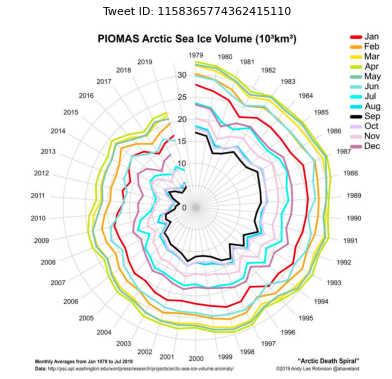
\includegraphics[width=0.4\textwidth]{images/good1.png} 
    \hfill
    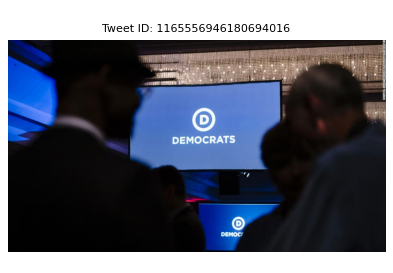
\includegraphics[width=0.4\textwidth]{images/good2.png}
    \caption{Examples of well-aligned predictions (Case C on left, Case D on right).}
    \label{fig:good_cases}
\end{figure}

\subsubsection*{Case C: Tweet ID 1158365774362415110}

\noindent\textbf{Text Snippet:}
\begin{quote}
\#Arctic sea ice volume broke another record minimum for July ... less than half \\
of what it was 20 years ago. \#climatechange \#climatecrisis \#dataviz
\end{quote}

\noindent\textbf{Aggregated Reply Distribution (multiple replies):}
\[
\begin{aligned}
\{\text{anger: } 0.0768, \quad \text{fear: } 0.1475, \quad \text{surprise: } 0.2777, \\
\text{disgust: } 0.1378, \quad \text{sadness: } 0.1090, \quad \text{joy: } 0.2511\}
\end{aligned}
\]

\noindent\textbf{Our Predictions (Text-only):}
\[
\begin{aligned}
\{\text{anger: } 0.1557, \quad \text{fear: } 0.1377, \quad \text{surprise: } 0.2135, \\
\text{disgust: } 0.1306, \quad \text{sadness: } 0.2068, \quad \text{joy: } 0.1558\}
\end{aligned}
\]

\noindent\textbf{Our Predictions (Image-only):}
\[
\begin{aligned}
\{\text{anger: } 0.1074, \quad \text{fear: } 0.2742, \quad \text{surprise: } 0.2789, \\
\text{disgust: } 0.1031, \quad \text{sadness: } 0.1066, \quad \text{joy: } 0.1298\}
\end{aligned}
\]

\noindent\textbf{Our Predictions (Multimodal):}
\[
\begin{aligned}
\{\text{anger: } 0.0992, \quad \text{fear: } 0.2918, \quad \text{surprise: } 0.2525, \\
\text{disgust: } 0.0917, \quad \text{sadness: } 0.1198, \quad \text{joy: } 0.1450\}
\end{aligned}
\]

In total, there were \textit{several distinct replies}, reflecting a wide range of sentiments. Some expressed concern (\textit{fear, sadness}), others surprise or disgust at the data, while certain replies maintained an optimistic or grateful tone (\textit{joy}):

\begin{quote}
\emph{``Great work—even if it highlights a worrying trend,''} \\
\emph{``The planet \& all that inhabit it are in a world of trouble...''} \\
\emph{``Thank you very much, I have been producing it every month [...] hoping people will notice, think, and act...''}
\end{quote}

This naturally yields a \textbf{higher entropy target distribution}, with each of the six emotions receiving non-trivial probability. Crucially, the KL-divergence loss encourages the model to match this spread. 
\newline

Overall, both the text-only and image-only predictions show varied emotion assignments; text-only dedicates a larger fraction to \textit{anger} and \textit{sadness}, while image-only shifts more heavily to \textit{fear} and \textit{surprise}. However, by combining both modalities, the multimodal system manages to produce a distribution that remains relatively balanced across the top four or five emotions. Indeed, our multimodal system successfully produced a more balanced distribution—resulting in lower KL divergence and better performance overall.

\subsubsection*{Case D: Tweet ID 1165556946180694016}

\noindent\textbf{Text Snippet:}
\begin{quote}
Democratic National Committee votes against allowing 2020 candidates \\
to participate in a climate change debate [URL]
\end{quote}

\noindent\textbf{Aggregated Reply Distribution (multiple replies):}
\[
\begin{aligned}
\{\text{anger: } 0.2326, \quad \text{fear: } 0.0911, \quad \text{surprise: } 0.1422, \\
\text{disgust: } 0.2849, \quad \text{sadness: } 0.0885, \quad \text{joy: } 0.1607\}
\end{aligned}
\]

\noindent\textbf{Our Predictions (Text-only):}
\[
\begin{aligned}
\{\text{anger: } 0.1660, \quad \text{fear: } 0.1510, \quad \text{surprise: } 0.1761, \\
\text{disgust: } 0.1281, \quad \text{sadness: } 0.1922, \quad \text{joy: } 0.1866\}
\end{aligned}
\]

\noindent\textbf{Our Predictions (Image-only):}
\[
\begin{aligned}
\{\text{anger: } 0.1749, \quad \text{fear: } 0.1821, \quad \text{surprise: } 0.2258, \\
\text{disgust: } 0.0994, \quad \text{sadness: } 0.0946, \quad \text{joy: } 0.2232\}
\end{aligned}
\]

\noindent\textbf{Our Predictions (Multimodal):}
\[
\begin{aligned}
\{\text{anger: } 0.2084, \quad \text{fear: } 0.1822, \quad \text{surprise: } 0.1753, \\
\text{disgust: } 0.0910, \quad \text{sadness: } 0.0857, \quad \text{joy: } 0.2575\}
\end{aligned}
\]

Here, we see a diverse mixture of emotions across the replies—many users felt \emph{anger} or \emph{disgust} (finding the decision frustrating), a few expressed \emph{surprise}, and others found \textit{joy} or positivity in certain commentary:

\begin{quote}
\emph{``This is stupid,''} \\
\emph{``Why let us hear what each [candidate] has to contribute?''} \\
\emph{``I appreciate their effort in losing as many elections as possible...''}
\end{quote}

Since multiple replies contributed to the final distribution, it exhibited relatively high entropy. Our text-only predictions emphasized \textit{sadness} (19.2\%) more than the aggregated replies, while our image-only model gave heavier weight to \textit{fear} (18.2\%) and \textit{surprise} (22.6\%). Ultimately, the multimodal approach balanced these signals, producing a smoothed distribution with strong peaks in \textit{anger} (20.8\%) and \textit{joy} (25.8\%), aligning well with the diverse nature of user replies.
\newline

Hence, in cases of \textbf{diverse or high-entropy user replies}, the model excels at mimicking the broad emotional composition, lowering KL divergence.

\vspace{1em}
\subsubsection*{Illustration of Noisy or Poorly Written Replies}

While many replies are coherent, we also observed \emph{poorly written} or difficult-to-parse responses. Such messages can introduce errors or unusual probability spikes when aggregated. For instance, consider a few actual examples from our dataset (unedited):

\begin{quote}
\emph{``BASIL AMAELO????''} \\
\emph{``nibiu close eath''} \\
\emph{``dnc no commentsame trough''} \\
\end{quote}

The model sometimes interprets these short, ambiguous, or grammatically unclear statements as expressing \textit{anger} or \textit{disgust}, based on certain keywords or negative connotations (e.g.\ ``no comment'' or random capital letters). Other times, the mention of a presumably serious topic (``energy production'') may inflate \textit{fear} or \textit{surprise}. When such replies are averaged with others, they can skew the final aggregated distribution and increase error—particularly if there are only a few total replies.

\bigskip


\subsection{Key Findings}
\subsubsection*{Impact of Reply Entropy on Model Predictions}
The variability in human reply distributions plays a critical role in model alignment with soft labels:
\begin{itemize}
    \item \textbf{High Entropy $\rightarrow$ Better Alignment:} When replies exhibit diverse emotional reactions (e.g., Cases C and D), the model effectively replicates the distribution, accommodating overlapping sentiments such as fear, disgust, sadness, and joy.
    \item \textbf{Low Entropy $\rightarrow$ Greater Divergence:} When replies predominantly express one or two emotions (e.g., Cases A and B), the model tends to over-distribute probabilities, leading to prediction "flattening" and higher KL divergence. This occurs despite strong human consensus on emotions like fear, sadness, or surprise.
\end{itemize}

Additionally, the training objective plays a crucial role in shaping the model’s behaviour:
\begin{itemize}
    \item The \textbf{KL divergence loss discourages overconfidence}, ensuring that when human responses are uncertain or divided, the model produces softer distributions.
    \item However, when replies overwhelmingly agree on a single emotion, the model often spreads its predictions too broadly, underestimating the true peak.
\end{itemize}

\subsubsection*{Text and Image Ambiguity: A Secondary Factor}
While sarcasm, slang, or ambiguous imagery can contribute to misclassifications, these factors were not the primary drivers of errors. Instead, \textbf{the shape of reply distributions and the model's training objective exerted a stronger influence}, as confirmed by both numerical trends and qualitative inspection of user responses.



\section{Conclusion}
\label{sec:conclusion}

Fine-tuning provides marked improvements over zero-shot classification for both text and image modalities, significantly reducing KL divergence and increasing cosine similarity scores. The additional benefits from multimodal fusion confirm that integrating visual and textual information can yield more robust representations.

However, these gains also highlight emerging challenges—such as minority label collapse and over-reliance on dominant emotional categories—that warrant deeper exploration. In the next chapter, we delve into a comprehensive analysis of these issues, examining the interplay between distribution-level metrics and instance-level accuracy, as well as the broader implications for real-world emotion classification tasks.





